\documentclass[UKenglish]{ifimaster}
\usepackage[utf8]{inputenc}
\usepackage[T1]{fontenc,url}
\urlstyle{sf}
\usepackage{babel,textcomp,csquotes,duomasterforside,varioref,graphicx}
\usepackage[backend=biber,style=apa]{biblatex}
\usepackage{pifont}


\usepackage{amsmath,amssymb,amsfonts}
\usepackage{algorithmic}
\usepackage{textcomp}
\usepackage{xcolor}
\usepackage{textgreek}
\usepackage{float}
\usepackage{graphicx}
\usepackage{comment}

\graphicspath{ {./pictures/} }



% TODO: laste ned APA pakke

\raggedbottom

\title{Interactive meaning-making in a museum context}
\subtitle{How can one design meaningful interactive experiences in a museum space that addresses sustainability?}
\author{Silje Marie Flaaten}


%name of your bib file(s)
%\addbibresource{zotero.bib}
\addbibresource{bibliography.bib}

\begin{document}

\duoforside[dept={Department of Informatics}, program={Informatics: design, use, interaction},long]

\frontmatter{}
\chapter*{Acknowledgements}
Thanks, thank you, thanks, thanks, thanks, thank you thank you, wow such support, thanks, thanks, thanks I feel so supported, thanks thanks, thank you, thank you

% First of all I want to express my thanks and gratitude for my superhero-supervisor Joshi. Thank you for your patience, new perspectives and good talks throughout the thesis project. Your guidance, affirmations, and critical eye have been crucial for the coming-together of the project and report!

% Dear Janni and Sandra, thank you for the collaboration efforts throughout the thesis project! It has been a joy visiting museums and doing fieldwork with you. Talking, reflecting and discussing with you have shaped and driven forward the scope and interest of this thesis in so many ways. I am so proud of the work we have done together, and how the three thesis's complement each other. 

% Thank you Adrian for dragging me out of the university and making me disconnect from the pc and thesis from time-to-time, or else I would have turned proper mad scientist. Thanks for geeking out on the Timeless Way of Building and on The Phenomenon of Life with me. These conversations have not only fulfilled a lot of the missing pieces in the thesis, I see us growing so much as designers simultaneously. Now lets go surfing!!

% And of course, thank you to all of my ifi-friends. Studying during a pandemic and war in Europe has not been easy on any of us, but we have done the best we could nonetheless. Special thanks to my peeps from the coffee-break gang, and the design-folks on the 7th floor for making the last two years such a good time. I have looked forward to seeing you every day. Thank you for all the fun nights out, the weekly climbing sessions, the long lunch breaks and for being supportive in all the right ways when things have been difficult.

% Thank you to my friends and family for checking in on me, sending heartfelt words and thoughts my way.

% This thesis has forever changed museum-going for me. I have found it immensely fun to deep-dive into the museum domain, which I did not have much knowledge on beforehand. I am glad to have derived new skills and perspectives that I will take with me in future designer practise. Hope that those of you who find the thesis interesting do the same. Ok hehe bye, enjoy the reading! -Silje 

%\chapter*{Abstract}
%This thesis reports from an analysis of 21 interactive installations, seeking to answer how one can design meaningful interactive experiences in a museum space that addresses sustainability. Throughout the thesis we present the creation of a theoretical framework to identify and generate data that makes visible dialogic behaviour, suitable for analysing the exhibition and judge how the installations stimulate dialogue, conversations or reflections. This is how the thesis frames and capture meaningfulness in exhibition design. We then present a list of patterns that have objectified meaningfulness through a description of dialogical behaviour between the visitor and the interactive installation. The main findings in this thesis is the theoretical framework, and the list of patterns derived from using the framework.

\tableofcontents{}
\listoffigures{}
% \listoftables{}

% \chapter*{Preface}
% 
my motivation and interest for sustainability, museums and interaction design?


\mainmatter{}
\part{Introduction}
\chapter{Aim of study}
\section{Museum's role in society}

In the recommendation letter report \emph{“Museums in the society - trust, things and time,”} the standing committee of Cultural Affairs presents the overall political direction for Norwegian museum policy towards the year 2050 (Figure 1.1). The report establishes that Norwegian museum institutions take aim to express both historical and current developments in society. And that museum institutions play an important role in our own time’s understanding of ourselves - both who we have been, who we are, and whom we want to be \autocite[p. 7]{melding23}. Modern museum operations aim to actively turn to the general public with the objective to build and share knowledge, increase enlightenment and cultivate cultural capital. Where the early museum institutions, first and foremost, were accessible to a small number of privileged class members, it is now expected that museums purposefully reach out to be open and accessible to all residents and age groups \autocite[p. 14]{melding23}. In Norway, museums are increasingly understood as both knowledge and social institutions, where dissemination and exhibition practice are curated accordingly. At the same time, museums have emerged as an alternative learning arena for school children, first regarding history teaching, but later in many other subject areas as well. In a society where polarization and public debate are intensifying, arenas that have the public's confidence in being able to nuance and disseminate different perspectives are needed \autocite[p. 7]{melding23}.

\begin{figure}[H]
\centering
\includegraphics[width=8cm]{pictures/Introduction/stortingsmelding_hoykant.png}
\caption{The recommendation letter report Meld.St.23 \emph{“Museums in the society - trust, things and time"}} {\autocite[p. 1]{melding23}}
\end{figure}

There is a saying among historians that \emph{"the past teaches us about the present"}. History is a subject that is extra rich in perspectives, explanations, and ideas about how people have lived, thought, and acted. It positions us to see patterns that might otherwise be invisible in the present – thus providing a crucial perspective for understanding and solving current and future problems \autocite{UW_website}. Being a knowledge institution, museums have the power to both define and showcase relevant historical events as a perspective to inform present societal issues and debates. 

% Klimahistorie: eget avsnitt?

% Skiftet til museene handler ikke bare om å fornye seg, altså appellere til en bredere målgruppe, men det handler om å "henge med i tiden", og klare å forankre dagsaktuelle debatter/ samtaler med et faglig, vitenskapelig korrekt, blikk.

\section{Motivation}
Short orientation on motivation for topic. Say something about \emph{why} meaningfulness.


\section{Research question and framing of project}
The aim of this study is to gain insight to try answer how one can design interactive meaningful experiences in a museum space that addresses sustainability. To understand this, several installations have been analysed as a way to objectify \emph{meaningfulness} as a quality that you can design for. In the HCI community, meaningfulness is recognised as a quality in made products or artefacts that not only make people more efficient and effective, but through use in activities, relationships, routines, and rituals, become meaningful \autocite{zimmerman_designing_2009}. This thesis fills a gap in the literature where the term is explored through a museum context for experience designers, trying to objectify meaningfulness as an interactive quality that support dialogic behaviour between visitors and installations in museums. Special attention has been given to museums that aim to encourage social action, like climate consciousness or climate action as examples of meaningful behaviour museums addressing contemporary discourses want to encourage.

This thesis aim to answer how one can design meaningful interactive experiences in a museum space that addresses sustainability. This is attempted through objectifying meaningfulness as a quality that you can design for in a museum, by identifying and analysing dialogic relations between visitor and installation.

In my attempt to answer how one can design meaningful interactive experiences in a museum space that addresses sustainability, I have composed concepts from three theoretical approaches to place-centred design to make my own theoretical framework to better understand interactive artefacts dialogic qualities and museum experience design. This attempts to answer how museum spaces can look at their respective installations and judge whether or not they stimulate the visitor to dialogue. The hypothesis is that there lies value for the museum to judge whether or not their installations promote dialogue.

\section{Scientific contribution}
The thesis investigates how interactivity can support visitors meaning-making in a museum space. The hypothesis is that an interactive installation or experience have the potential to reinforce the message conveyed in a manner that give rise to thought-provoking or significant reflections that last long after the museum visit. Something which also encompass the power to deliberately stimulate visitors lifestyle choices or actions after the museum visit, in compliance with the museums agenda and vision. 

\break
\section{Chapter overview}
The thesis is divided into three parts; Introduction, Design Process, and Review/ Evaluation. The (report) structure reflects the methodological nature of doing Research through Design, where the Design Process is evidence of the practical activities shaping the thesis project. If not referenced otherwise, all pictures in this thesis come from a shared photo library the research buddies and I have built up and accumulated during fieldwork. The same goes for illustrations. If not referenced else-wise, they are illustrated by me.

\subsubsection{Chapter 2: Modern museums and sustainability}
Chapter 2 is a focused selection of terminology and concepts attained from the literature review that has been conducted throughout/during the thesis project. It is structured in the hope that designers interested in the topic can adopt the concepts as a vocabulary and mean of understanding some of what goes on in the museum world. The literature review has nonetheless been crucial for the thesis evolution. On the one hand, it has influenced the research framing and interest, shaped and refined the research question, and leveraged the vocabulary when documenting/ recounting an exhibition- and installation experience. While on the other hand, it has influenced the convergent and divergent thought process when going in and out/back-and-forth of practical and theoretical work, the designer role, and the researcher role.

\subsubsection{Chapter 3: Three approaches to place-centred design }
Chapter 3 is a continuation of the literature review. Where Chapter 2 indirectly affect the thesis evolution, Chapter 3 present three theoretical approaches that have formatively guided e.g. data-gathering guides during fieldwork, both for observations, interviews and analytical critique.

\subsubsection{Chapter 4: A new way of designing for meaningfulness?}
In Chapter 4, we build upon and borrow concepts from the three theoretical approaches presented in Chapter 3, in the making of a new theoretical framework as a proposal of a new way of designing for meaningfulness.

\subsubsection{Chapter 5: Methodology}
In Chapter 5 you can read on the methodological approach to Research through Design adopted through this thesis.  

\subsubsection{Chapter 6: Design Process}
In Chapter 5 you can read on the methodological approach to Research through Design adopted through this thesis.  


\subsubsection{Chapter 7: Analysis}
\subsubsection{Chapter 8: Discussion}
\subsubsection{Chapter 9: Conclusion}




\chapter{Modern museums and sustainability}
This chapter gives an introduction to literature from the museum field, starting with the ongoing transitional shift to a \emph{new} museology. The chapter will then introduce concepts and terms from exhibition and dissemination practise to extend the vocabulary for talking about museum subjects and roles. Then we will progress into sustainability as a topic representative of a contemporary discourse being addressed in a museum. The chapter is then rounded off with literature on the application and use of technology and interactive installations in "modern museums."

\section{The new museology}
In 1989, Peter Vergo coined the term \emph{the new museology} in a book bearing the same name. Museology is the study of museums, their history and underlying philosophy, and the various ways in which they have during the passing of time, been established and developed \autocite[p.1]{vergo_museology_1989}. Vergo argues that beyond the physical material like handouts or information panels, there is a subtext comprising diverse and often contradictory strands woven from the intellectual, political, or educational preconceptions of the museum stakeholders, e.g. the museum director, the curator, the scholar or the designer \autocite[p.3]{vergo_museology_1989}. Rather than old considerations like administrative tasks, conservation techniques, financial well-being, or, success or neglect in the eyes of the public, the subject matter that should be more questioned or discussed should be more concerned with the museums \emph{purpose} rather than museum \emph{methods} \autocite[p.3]{vergo_museology_1989}. Vergo would therefore define the \emph{new} museology simply as a state of widespread dissatisfaction with the \emph{old} museology considerations. "Unless a radical re-examination of the role of museums within society takes place", Vergo declares that museums in this country (referring to the UK), and possibly elsewhere, may likewise find themselves dubbed 'living fossils' \autocite[p.4]{vergo_museology_1989}.

Throughout this thesis project, it has become quite evident that Norwegian museums are making efforts to renew themselves and embrace the possibilities that interactive exhibition curatorship could encompass. Moreover, that interactive and audiovisual elements are almost self-evident parts of the exhibition strategies in Norwegian museums \autocite[p. 59]{melding23}. Compared with other countries' museums, e.g., the Louvre in Paris, France, which could be an example of Vergo's traditional museum or old museology tradition, where the art represents or at least is very tightly coupled with the french cultural heritage and national identity. This means conservative voices in public can stand in the way of renewal or change, making the transformative strategies more elongated. However, literature agrees that the museum world has undergone radical changes since the 1970s- and 80s. \emph{"Political and economic pressures have forced its professionals to shift their attention from their collections toward visitors. Whereas in the past, the museum tended to be exclusive and elitist, signs of a progressive opening-up and greater accessibility have appeared. A climate of increasing reflexivity within the profession is identified as a 'new museology'."} \autocite[p. 84]{ross_interpreting_2015}.

\subsubsection{Museum experience design}
Recent literature in the HCI field concerned with museums agrees that the museum world is rapidly changing from being collection-centered to being community-centered and for the public \autocite[p. 1]{vermeeren_museum_2018}. And that museums have become a place for education and learning, dialogue and debate \autocite{hein_1998}, \autocite{hooper_1994}, \autocite{Roberts_1997}. New ways of involving the public more meaningfully have emerged, but there is still much to uncover; experiences in museums have become more engaging by extending the experience beyond the physical visit. \autocite{vermeeren_museum_2018} presents four key themes relevant for designers concerned with experience design in museums:

\begin{itemize}
    \item Engaging the public,
    \item Cultivating diverse audiences,
    \item Availing ourselves of the benefits of digital technology,
    \item and, Leveraging museums’ roles as players in larger economic and cultural ecosystems.
\end{itemize}

This thesis and its research inquiries positions itself in the first key theme presented; engaging the public, with the goal to understand more about how one can design meaningful interactive experiences in a museum space. \emph{Too often we (the museum) prioritize our mandate to hold and protect our collections and stop short of making them relevant to today’s audiences, real or potential. Too often we are zoomed way too far in on our objects, and lose sight of what people less invested might know, think, or want from us.}\autocite[p. 1]{vermeeren_museum_2018} In light of this, \autocite{vermeeren_vincent_2018}'s case on \emph{Becoming Vincent} is instructive where it among the findings is implied how "the importance of and attention to content is related to the increasing value associated with craftsmanship, in the belief that this will provide a real, genuine, and authentic experience" \autocite[p. 298]{vermeeren_vincent_2018}. "When we pull our focus back from the individual museum and its obsession with its objects, we find a larger community outside that is largely indifferent to our obsessions, and needs a story, even a superstar, to motivate their interest" \autocite[p. 1]{vermeeren_museum_2018}. "This is why storytelling can help turn any experience into a memorable and meaningful experience, by unlocking values that would otherwise be not so immediately recognizable by the listeners" \autocite[p. 299]{vermeeren_vincent_2018}. Then, "a struggle emerges between the museum’s role as protector of authentic objects and the “facts” around them and its role as a site of experiences—preferably extraordinary ones, because if not, why bother? "\autocite[p. 1]{vermeeren_museum_2018}. \emph{"So, while digital apps take us on mobile adventures and open up trails of wonder for some, the vast majority of our visitors still default to analog first and foremost. The more we can design for blended environments that mix the virtues of analog and digital affordances in mutually reinforcing ways to foster a context for meaningful engagement with museum objects, the better off we’ll be"} \autocite[p. 1]{vermeeren_museum_2018}. This show how the HCI community is increasingly interested in, and can benefit from, understanding more about how technology-use impacts the human experience of meaning and foster meaningful user experiences in museum contexts.

\section{Exhibition and dissemination practise}
In this section, I will present terms and concepts to explain what I mean when I talk about exhibition and dissemination practice. This lays the foundation for the vocabulary which I have adopted throughout the literature review and formatively guided data gathering and research inquiries. As supported by the Oxford dictionary of English definitions of \emph{exhibition} and \emph{dissemination} in Figure 2.1, the way exhibition and dissemination practice is understood and used in this thesis is as follows: dissemination as in the act and action of spreading information in the context of an exhibition displaying works of art, items of interest, and interactive installations in a museum.

\begin{figure}[H]
\centering
\includegraphics[width=14cm]{pictures/background/exh_diss.png}
\caption{Exhibition and dissemination practice}{\autocite{Oxford_dictionary}}
\end{figure}

\subsection{Understanding the museum discourse}
Coming into this thesis project, I knew very little about how a museum worked or functioned. Wanting to learn more about how narrative play a part in telling a story and conveying a message, I came across \autocite{Miekebal_book}'s writings on cultural analysis and discourses in the museum. Coming from a humanities background, she proposes a perspective on what differentiates the “new” from the “old” museology. According to her, the museum is seen as a discourse and the exhibition as an utterance within that discourse. She calls this a discursive perspective. By bringing this discursive perspective to the museum, it has the possibility to "deprive the museal practice of its innocence, and provide it with the accountability it and its users are entitled to" \autocite[p. 214]{Thi_book}. Part of her argument and critique is that politics come straight out of, or more precisely are bound up with, the museal discourse \autocite[p. 214]{Thi_book}. To deal with this, she suggests a threefold direction for museology researchers. First, she suggests systematically analyzing the narrative-rhetorical structure of the specific museum to refine the categories and deepen insight into their effects. Secondly, she suggests looking at the connection between the museal discourse and the institutions' foundation and history. Thirdly, she sees the need to do a self-critical analysis of the museal discourse as a consequence of the nature of discourse. \autocite{Miekebal_book} argue that in the study of museums, one should look at the museum and question:

\begin{itemize}
    \item What museum fiction do the museum tell? 
    \item Who is speaking the museum fiction?
    \item Who is the expository agents?
    \item And what is the museums expository agency?
    \item What is spoken? 
    \item Is the museum telling, showing or showing off?
\end{itemize}

These concerns make up the foundation for seeing the museum for what it is and what it presents up against what it represents. According to \autocite{Miekebal_book}, the museum itself is the expository agent. Putting forward the expository agent that “speaks” the text in the verbal panels transforms the one with a commentary on the other. Making it possible to judge whether the fiction of the museum's expository agency aligns with the expository agent's vision or not. Different museums speak different fictions, e.g., art, science, cultural heritage, but what these fictions have in common is that they show their objects, not their own hand or voice \autocite{Miekebal_book}. The way she sees it, showing, if it refrains from telling its own story, it becomes showing off. The displays can then point at their discourse as a sign system put forward by a subject, and one can look for issues of cultural moralism or cultural imperialism. Her studies are concerned with and derived from the context of looking at ethnographic museums that display ethnic objects and artefacts representing cultures and cultural properties from the past. She raises the question if former colonists are entitled to hold onto objects taken by their ancestors from former colonies, or should they give these back to the country of origin to the ancestors whose inhabitants were their original owners? This is a debate totally out of scope for this thesis but relevant in understanding the implications a discourse can have. The way I see it, sustainability and the climate crisis is a complex discourse that shares some of the same dynamics that the colonist- discourse does in terms of the uneven distribution of the cause-effects of climate change — potentially resulting in cultural moralism. As we can see from the Oxford dictionary of English in Figure 2.2, the way \emph{discourse} is understood and used in this thesis is to reference a topic or theme in the museum context, talking about either the exhibition discourse or the museum discourse.

\begin{figure}[H]
\includegraphics[width=12.5cm]{pictures/background/discourse.png}
\caption{Museum discourse}{\autocite{Oxford_dictionary}}
\centering
\end{figure}
 
I think this critical discourse-oriented perspective is necessary in a museum context or exhibition space addressing sustainability because the intention of making a meaningful interactive experience is also about strengthening the message conveyed by the museum. Both the designer and especially the museum's expository agents need to be aware of and able to answer the moral and ethical questions raised regarding what the message they convey, actually conveys. And that the act of strengthening that message through interactivity sends people out of the museum with reflections and thoughts that hopefully leads to social action like climate action or higher climate consciousness. There has been increasing interest in the HCI community in considering how technology-use impacts the human experience of meaning \autocite{light_design_2017}, questioning what a good design for an existential crisis is. "In the Anthropocene age, shocks of all kinds are raising questions about the future and value of humankind." \autocite[p. 723]{light_design_2017}. Light et al. argues that while there are increasing indifferences to the ecological consequences of the world, ultimately there is a growing sense that, without fast action at every level of society, we cannot outrun crisis \autocite[p. 723]{light_design_2017}. "Institutional humiliation comes in many digital guises", and Light et al. highlight the problem of techno-paternalism that nudges users toward behavior identified by others as positive, right or useful - an intensification of system efficiency at the expense of flexibility and the absence of empathetic hearing \autocite[p. 727]{light_design_2017}. Can this be an example of a modern-day concern for cultural moralism in museum exhibition and dissemination practice? 

Technologists and designers are implicated in this wave of change and uncertainty because the implications of the work they do, claims a stake in the production of futures \autocite[p. 723]{light_design_2017}. "As makers, we are practical people, as well as dreamers and theorists, and if there is no more “business as usual”, we can choose to have a role in producing alternative narratives for present generations of humans and those who depend on them, such as other species and unborn children." \autocite[p. 723]{light_design_2017}.

\subsection{Artefacts vs. artworks}
The very act of collecting has a political, ideological, or aesthetic dimension that cannot be overlooked. Vergo questions, "what makes certain objects, rather than others 'worth' preserving? \autocite[p. 2]{vergo_museology_1989}. "The original intention behind the establishment of museums was that they should remove artefacts from their current context of ownership and use, and insert them into a new environment which would provide them with a different meaning" \autocite[p. 6]{vergo_museology_1989}. "The essential feature of museums - and what differentiates them from the many extensive private collections which preceded them - was, at first, that the meanings which were attributed to the artefacts were held to be arbitrary; and, second, that the collections should be accessible to at least a portion of the public, who where expected to obtain some form of educational benefit from the experience" \autocite[p. 6]{vergo_museology_1989}. "A museum is an attractive object of study because it requires interdisciplinary analysis; it has the debate on aesthetics at its core, and it is essentially a social institution" \autocite[p. 202]{Thi_book}. The heritage museum conserves and exhibits artefacts, while the art museum, works of art. It seems obvious what differs between the artefact vs. the artwork, yet they differ in what they represent. Both the artefact and the artwork is charged with cultural meaning. It tells us about a more extensive cultural situation, e.g., aesthetic conceptions or world views, conceptions of representations, or the social relevance of art. However, these meanings are only yielded if we can “read” them or is put in some context that illuminates the cultural meaning \autocite[p. 206]{Thi_book}.

The term artefact suggests a man made object charged with cultural meaning which can, if studied carefully, offer us information on the society in which it has been created \autocite[p. 205]{Thi_book}. The difference between the artefact according to the above definition and the common idea of art is that the former takes for granted what the other represses: the possibility of cultural difference. Instead, artworks are viewed as standing for an aesthetic, and is therefore considered metaphors, transferring their specific aesthetic to the one current sufficient to make the work “readable” as art, regardless of what it could tell us about the culture it comes from \autocite[p. 206]{Thi_book}. While the ethnic artefact, in contrast, is first and foremost considered to be a representative of the larger context of the culture it comes from \autocite[p. 206]{Thi_book}. Hence, it is not a metaphor but a synecdoche. Synecdoche is the figure of rhetoric where an element, a small part, stands for the whole simply by virtue of its being a part of that whole \autocite[p. 206]{Thi_book}. Thus the artefact is only readable as culture, no matter what aesthetic qualities it may also have.

% something about interactive artefacts, artworks or installations?


\subsection{The curatorial function}
% Kanskje introdusere med noe sånn: Fra boken (thinking about exhibitions), kapittel 1 skriver (Carmen?) om kuratorens rolle i museet. 
The curator are, above all, the institutionally recognised experts of the art-world establishment, whether they operate inside an institution or independently. More than art critics or gallery dealers, they establish the meaning and status of contemporary art through its acquisition, exhibition, and interpretation \autocite[p. 22]{Thi_book}. To a greater extent than other art-world professionals, curators additionally depend on an established infrastructure to support their efforts. This infrastructure includes institutionalised networks, such as those provided by museums, galleries, or alternative spaces; financial sponsors, whether public, private or corporate, and teams of technical or professional experts \autocite[p. 22]{Thi_book}. Curators are the sanctioned intermediaries of these institutional and professional networks on the one hand, and; artists and audiences on the other. The curatorial function is, this, inherently restricted by the interests of the larger or more powerful groups and constituencies in the museum \autocite[p. 22]{Thi_book}.

By selecting, framing and interpreting peripheral art in exhibitions and exhibition catalogues, for instance, art curators can claim to be shaping a more democratic space where specific cultural groups can recognise themselves \autocite[p. 23]{Thi_book}. As the debates of recent years have shown, “identity” is not an “essence” that can be translated into a particular set of conceptual or visual traits. It is, rather a negotiated construct that results from the multiple positions of the subject vis-a-vis the social, cultural and political conditions which contains it. How then, can exhibitions or collections attempt to represent the social, cultural and political complexities of groups without reducing their subjects to essentialist stereotypes? \autocite[p. 23]{Thi_book}.

This situation places the cultural broker at the very core of a contradiction: on one hand, she can be credited for helping to tear down artworld hierarchies, seemingly democratizing the space for cultural action; on the other hand, in a market scenario where “identity” can only be a reductive construct, the framing and packaging of images of the collective self can only result in a highly delusionary enterprise \autocite[p. 23-24]{Thi_book}. The tensions of this contradiction confront art curators with a dilemma; where should they position themselves vis-a-vis the identities of the groups they claim to respect? \autocite[p. 24]{Thi_book}.

\subsection{Dialogical engagement}
"Museums started off as institutions focusing on collecting and preserving objects, open for the public to come and watch. The primary purpose for visitors to come to the museum was to see the original objects. A first notable shift saw the museums move from a collection focus to a visitor focus and from a mission for objects preservation and access provision to a mission of offering meaningful engagements with the collection and rewarding learning experiences for their public. The concept of ‘museum experience’ is the pinnacle of this historical shift, as it implies a focus on the visitor and connections between visitor and objects rather than a focus on collections. In the course of time, new types of museum experiences gradually emerged. The degree of sophistication and immersion increased exponentially when experiences started to be enhanced by the integration of interactive and digital media. In many science and technology museums, for example, visitor engagement and participation are uplifted through the use of new media (e.g. video games, interactive installations and other forms of edutainment) to encourage visitors to engage with the content on exhibit, to experiment with the techniques on show and to appropriate the visiting experience by making it meaningful and memorable. This trend is being adopted also by art museums, where it is by definition more difficult to let visitors experiment with the collections." \autocite[p. 3]{vermeeren_museum_2018}.

\begin{figure}[H]
\includegraphics[width=6cm]{pictures/background/dialogic.png}
\caption{'Dialogic' defined in the Oxford dictionary of English (UK).}
\centering
\end{figure}

\subsection{Museology and the Anthropocene}
% The Anthropocene refers to the present geological age, when humans are credited with having more impact on climate and planet than other factors combined.

In a call for publication and participation to the conference "The future of tradition in museology" organized by ICOFOM in Kyoto 2019, the same institutional change and questions concerning the future of museology that we just have read through the eyes of \autocite{ross_interpreting_2015}, \autocite{vergo_museology_1989} and \autocite{vermeeren_museum_2018}, is addressed. They present five directions to be considered worthy of further research, whereas two of them stand out in term of this thesis's research interest. \autocite[p. 4]{icofom_kyoto_2019}:

\begin{itemize}
    \item \textbf{Museological tradition vs global development and new technologies:} What role does museology play and what position does it take in relation to the rapid changes that are taking place? (...), e.g. will cyberspace out rule other spaces and materialities – (...), considering the return to extreme political positions and the “war” of information and knowledge?
    \item \textbf{Museology and the Anthropocene:} How can museology reduce the disastrous effect man has on our planet earth and our living conditions? How can museology help to bridge the gap between mind and matter – the gap that is the reason for the state of mankind right now – the belief that man is superior to nature and all other creatures? (...) So what impact should this insight bring to our dealing with museums, objects and collections, with a sustainable future in mind?
\end{itemize}

\begin{figure}[H]
\includegraphics[width=12.5cm]{pictures/background/anthropocene.png}
\caption{Anthropocene definition from the Oxford dictionary of English (UK).}
\centering
\end{figure}

\section{Museums communicating the science of climate change}

"One of the key terms today is learning in formal and informal contexts. Museums, too, are redefining their mission; instead of focusing on collecting and classifying, the emphasis is now on exhibition design and the museum as a place for communication and learning" \autocite[p. 8]{insulander_designs_2009}. 


"Social research underlines how the mass media frames and presents environmental change and risk in ways that become contested cultural constructs embedded in deep ideological structures" \autocite[p. 1]{salazar_mediations_2011}." While significant attention has concentrated on the mass media, less consideration has been given to examining the role of museums and science centres in communicating the science of climate change" \autocite[p. 1]{salazar_mediations_2011}. In the article "The mediations of climate change: museums as citizens media" \autocite{salazar_mediations_2011} looks at museums as cultural brokers around the public understandings of climate change. By engaging with recent conceptualisations around citizens and public media practises, Salazar proposes mechanisms through which the museum sector can act as change-agents in fostering a new form of public pedagogy that incorporates differing civic epistemologies around climate change education and action" \autocite[p. 1]{salazar_mediations_2011}.

\begin{figure}[h]
\includegraphics[width=10cm]{pictures/problem_sphere.png}
\caption{My representation of sustainability issues in museums}
\centering
\end{figure}


In a commentary by Richard J. Hebda, they look into the Royal British Columbia Museum (RBCM)’s voyage into the issue of climate change as an example of how museums can play a central role in addressing contemporary issues. Traditionally, museums have been a window to the past, "a place where the past lives" \autocite[p. 1]{hebda_article}. A lot of the issues and societal attitudes that are addressed in the commentary are still relevant today. Traditionally, human history and natural history has been seen as two solitudes that have been exhibited separately. A key appeal for the RBCM, a typical natural history museum to do a climate change exhibit, was to pursue the opportunity to link and integrate the two solitudes in a compelling and relevant manner \autocite[p. 2]{hebda_article}. They justify that the combining of the two is necessary because the exact same challenge is also central in the sustainability debate, at the core of the problem facing society today \autocite[p.2]{hebda_article}. In 2007 when the RBCM decided to make the climate change exhibition, the question of climate change was still a controversial issue \autocite[p.2]{hebda_article}. Addressing the increasing evidence and knowledge in terms of climate change and how it affects and is affected by humans, nearly all reputable scientists felt that change was under way and action was needed \autocite[p.2]{hebda_article}. The political and public atmosphere was foggy, as people did not know whom to believe, what information was science-based rather than rhetoric, and where real uncertainty lay \autocite[p.2]{hebda_article}. The RBCM saw a clear opportunity to dispel the fog and to enlighten their audiences \autocite[p.2]{hebda_article}.

\subsubsection{Changing Climate, Changing Attitude?}

"Many science museums and science centers now recognize their potential to arouse young peoples’ interest and awareness, and are starting to engage them in the climate change debate (e.g. Science Museum London, Australian Museum, Aquarium San Diego, American Museum of Natural History)" \autocite[p. 95]{gorr_changing_2014}. "Whereas some studies show evidence that museum and science center experiences may result in attitude change (Smithsonian Institution 2011; Spock 2000), there is evidence from a range of environmental-related exhibitions that initial changes in attitude and understanding fade after a couple of weeks because museum visitors tend to seek confirmation of their pre-existing attitudes and cling to erroneous beliefs (Adelman, Falk, and James 2000; Cakir 2008; Dierking et al. 2004)" \autocite[p. 95]{gorr_changing_2014}. "Some examples have even illustrated that attempts to increase people’s understanding of climate change enhanced skepticism and resulted in visitors’ total rejection of the issue (Jones 2009; Webster 2010)" \autocite[p. 96]{gorr_changing_2014}.

"Aiming to examine attitude changes in young people, the described study drew on general findings about attitude from social sciences and psychology. A closer look at the theory reveals that attitude is a highly complex and ambivalent term; for instance, a person may want to express both positive and negative attitudes toward the same object (Wood 2000). Whether an experience leads to longer lasting attitude change depends on numerous aspects such as motivation and attention (Petty and Cacioppo 1986). Motivation is mostly dependent on clarity and on the personal relevance of a message (Petty and Cacioppo 1979; Salazar 2011), or it may result from emotions, such as empathy and enjoyment (Roberts 1993)." \autocite[p. 96]{gorr_changing_2014}.



\section{Design as Meaning Making}

\autocite{kazmierczak_meaningmaking_2003} approaches design as an interface for meaning making, or simply the design of meaning. She see "meaning" as standing for a thought induced in the receiver, originated by contact with a design. According to her, design can be simple or complex in their material and conceptual structure but, as wholes, they are interfaces for meaning making \autocite[p. 47]{kazmierczak_meaningmaking_2003}. Borrowing from literature on cognitive semiotics, she proposes a model for design which relates physical form to cognition and comprehension rather than appearance and aesthetic. According to \autocite{kazmierczak_meaningmaking_2003}, there are two reasons why cognitive semiotics offers potentially good results; "First, it is focused on bridging the gap between form and meaning making or comprehension. Thus, its method of inquiry makes it well equipped for a discussion of symbolic-cognitive human phenomena such as communication. Second, it is compatible with the concerns of design regarding the construction of communications" \autocite[p. 47]{kazmierczak_meaningmaking_2003}. 

\begin{figure}[H]
\includegraphics[width=12.5cm]{pictures/background/semiotic.png}
\caption{Definition of Semiotic from the Oxford dictionary of English (UK).}
\centering
\end{figure}

Textual and written components are essential in any museum; 

I would argue that bringing cognitive semiotics (relating to signs and symbols) can be a useful perspective when working in/ designing for museums. It enables the designer to see the museum agenda and curatorial function up against the designed object, and when working with interactivity to emphasise dialogic qualities it should be useful to have the means to see, discuss and question the semiotic aspects of the designed object..... Museums that not only are 

\begin{figure}[H]
\includegraphics[width=12.5cm]{pictures/background/meaningful.png}
\caption{Definition of Meaningful from the Oxford dictionary of English (UK).}
\centering
\end{figure}


\begin{comment}

Hvordar forstår jeg bærekraft, og hvorfor mener jeg det er viktig?
Hvordan snakker andre om det, og hva må jeg få sagt til leseren om bærekraft?
Hvordan “angriper” jeg bærekraft temaet inn i denne oppgaven? 

\begin{figure}[h]
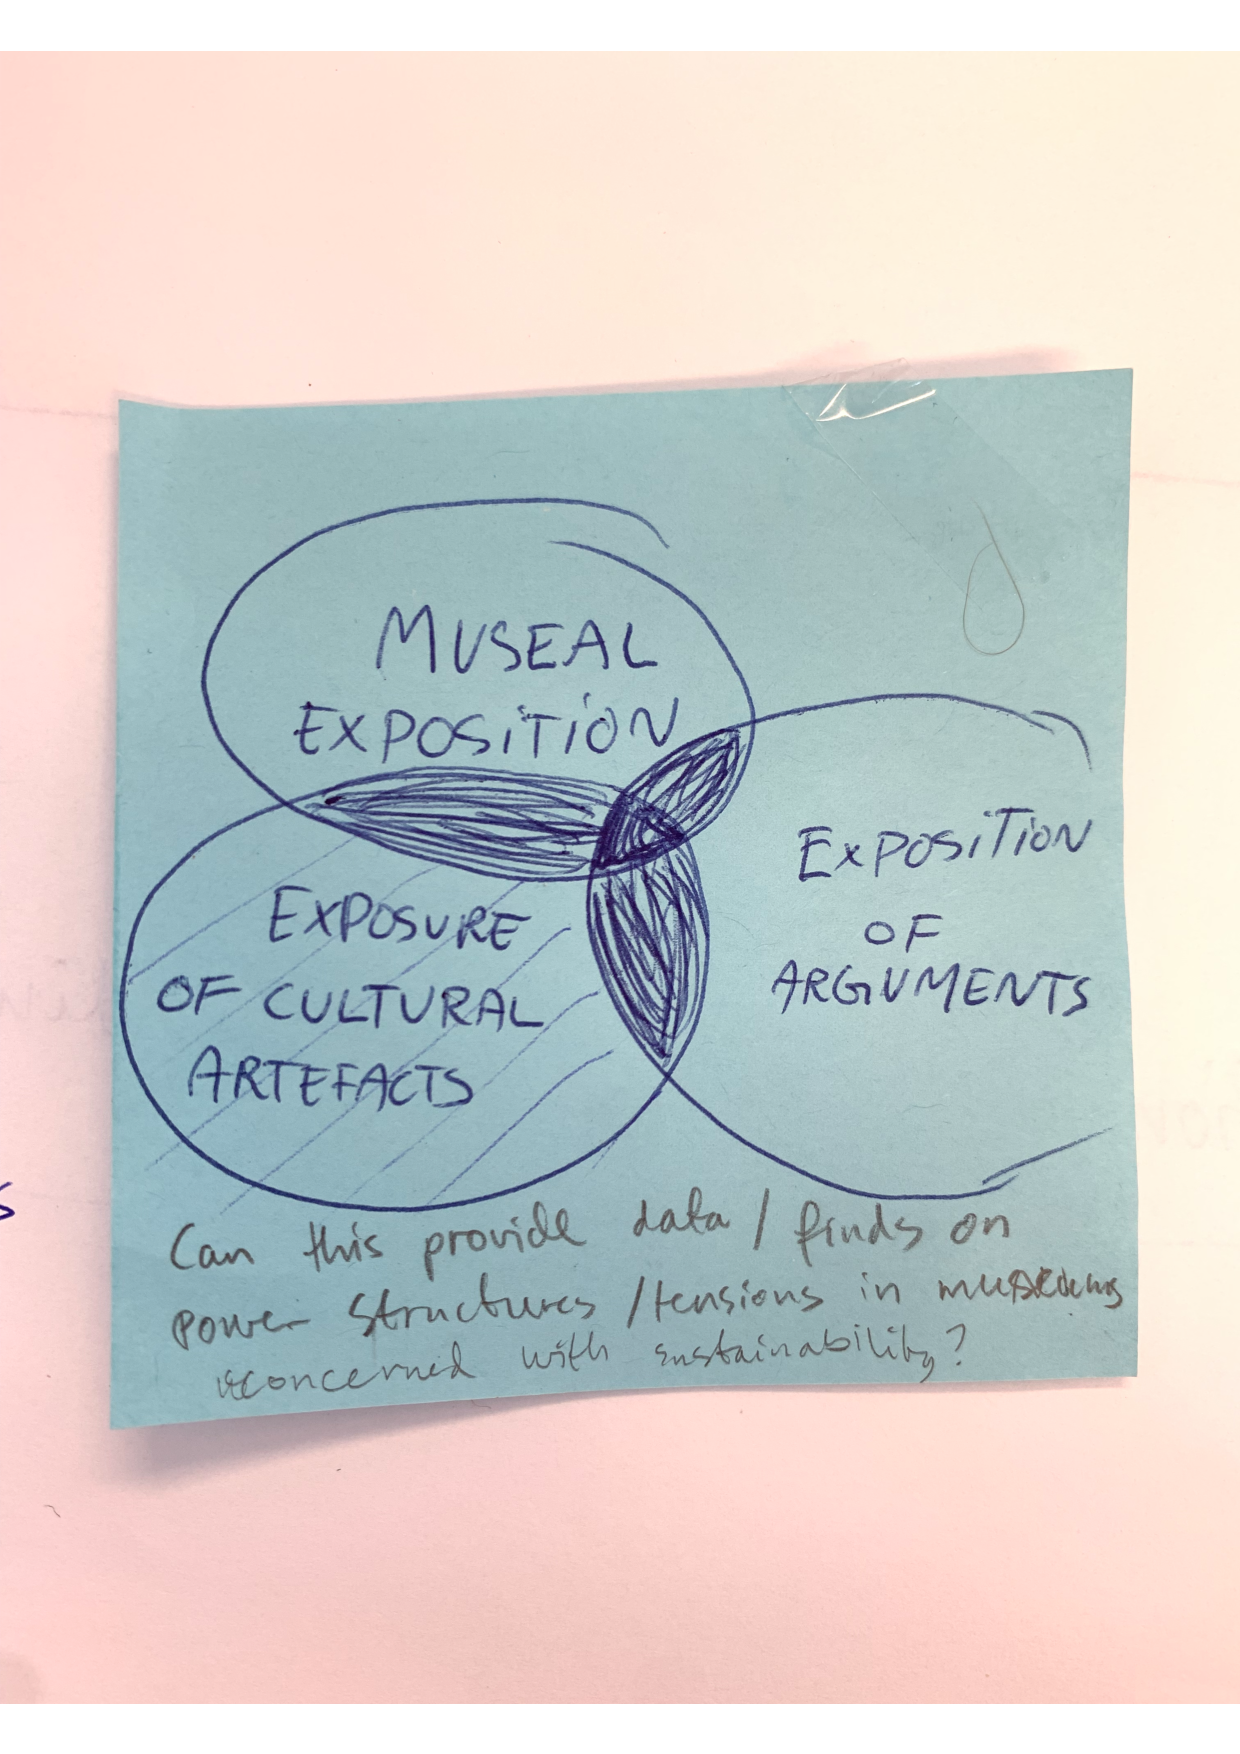
\includegraphics[width=8cm]{pictures/museumintersections.pdf}
\caption{Can the intersection between museal exposition, the museums exposition of arguments and their exposure of cultural artefact provide data or finds on power structures/ tensions/ imbalance in museums? Especially in terms of sustainability?}
\centering
\end{figure}

\end{comment}

% \chapter{Narrative theories}
% \section{Telling, showing, showing off}
\section{The value factory}
\section{The talking museum}

\subsection{Discursivity and cultural moralism}
Discursivity, most notably rhetoric imbricated with narrative is in effect a crucial aspect of the museum institution \autocite[p. 205]{Thi_book}, it is the core of the idea of exhibition.

The museum is an attractive object of study, because it requires interdisciplinary analysis, it has the debate on aesthetics at its core, and that it is essentially a social institution (Thi, p. 202) \autocite[p. 202]{Miekebal_book}. Mieke Bal account for and describe the issue of cultural imperialism in museums, exemplifying case studies related to natural history types of museums that conserves and display ethnic objects and artefacts representing cultures and cultural properties from the past. The ethnographic museum is clearly the most obviously politically charged institution, and it poses the immediate problem of cultural property and collective ownership (Thi, p. 202). It raises the question if former colonists are entitled to hold onto objects taken by their ancestors from former colonies, or should they give these back to the country of origin the ancestors of whose inhabitants were their original owners?

I think this (as a sort of ethical) perspective is necessary to have in this context, because the intention of making a meaningful interactive experience is to strengthen the message conveyed by the museum. Both the designer and especially the museum need to be aware of and able to answer moral and ethical questions in terms of what the message they convey actually conveys. And that the act of strengthening that impression in a greater way sends people out of the museum with reflections and thoughts that leads to social action (climate action, consciousness).


% \part*{\ding{167} \ding{167} \ding{167}}
% \part{Theory}
\section*{Structure}

The theory part consist of 4 chapters. Chapter 3, 4 and 5 presents the three theoretical theories I have used. And chapter 6 is a constellation of the three chapters and my proposal of a new theoretical lens to look at meaningfulness in a museum context.
\begin{itemize}
    \item Chapter 3: Hybrid place
    \item Chapter 4: Place as a dialogue
    \item Chapter 5: Sense-making
    \item Chapter 6: A new way to design for meaningfulness?
\end{itemize}
\par


\section*{Use of theory}
The use of theory is essential to any academic discipline. Before we embark on to the Theory chapters, it is necessary to go into how theory have been put to use throughout the thesis project. Theory takes researchers beyond observation and interpretation into the realm of shareable knowledge \autocite[p. 126]{beck_examining_2016}. It provides us with the means to structure knowledge, to evaluate and assess it, to construct it, and to share it \autocite[p. 126]{beck_examining_2016}. In a paper examining the practical, everyday theory use in design research, Beck and Stolterman discuss how researchers put theories to work in their written texts, and synthesise six models of "theory use". The models reflect the different ways researchers make use of theory beyond the commonly referenced uses of explanation, generalisation, prediction, and the like. And shows how theory can be used to motivate inquiry, contextualize research, shape research questions and guide methodology and analysis \autocite[p. 134]{beck_examining_2016}. The six models they propose is namely: no theory, theory as the object of study, theory as a contextualising tool, theory as a shaping tool, theory as a methodological tool, and theory as an analytical tool. Theory has primarily been put to use as a contextual tool, and as an analytical tool in this thesis.

\par \emph{Theory as an object} \par
"When a researcher develops an explanation of how or why some phenomenon occurs, they are engaged in theorizin - in a \emph{process}" \autocite[p.126]{beck_examining_2016}. The explanation itself becomes a theoretical \emph{object} \autocite[p. 126]{beck_examining_2016}.  


\par \emph{Theory as a tool} \par

Framing theory as a tool implies that a user uses theory for a particular purpose. Theory has been described and defined by many researchers in terms of its utility. It has been framed as a tool for explaining, describing, or predicting phenomena. It has been described in design research as a tool for "binding together" our knowledge of design practise and as a tool for "providing an understanding" of design writ large. \autocite[p. 127]{beck_examining_2016}. Similarly, theory is not necessarily an ideal tool for explaining reality in the same way that an analogy or metaphor might be. THeory, a tool for explaining, predicting, or describing, has structural properties conducive to other purposes as well. \autocite[p. 127]{beck_examining_2016}.


\par \emph{Theory as a reference} \par
Common definitions of reference include: the action of mentioning or alluding to something or the use of information to ascertain something. When theory is used as a reference, it most often appears in the introductory and/or background section of a given wrritten text \autocite[p. 128]{beck_examining_2016}. With this type of of theory use, researchers often reference frameworks and models \emph{instead} of referencing theory per se. Theory as a reference can perform several functions that may appear in concert or individually in a given research paper. For instance, a theory can be used to etablish the basis for a research project, to situate a text within a lineage, to establish the knowledge base of the writer, or to show connection to a community or school of thought. 
\par
(Mieke Bal narrative theories etc is an example of how  have used theory as a reference!)

\par \emph{Theory as a knowledge contribution} \par
Characterising theory as a \emph{knowledge contribution} suggests that it had not existed prior to the researcher's articulation of it. The researchers brought it into being by formulating their results such that they would be understood as a theory, for instance, as a set of constructs and their definitions, as well as a set of propositions about how the construct relate to one another. This formulation of a theory becomes a knowledge object. \autocite[p. 128]{beck_examining_2016}.





\chapter{Hybrid place}
In this chapter I will ....

\section{Designing a hybrid place}

Thanks to the development of ubiquitous and pervasive technologies, research focusing on the design of novel interactive artefacts has recently become more concerned with studying and understanding the spatial properties of the world \autocite[p. 159]{hybridplace_ciolfi}. Bringing technologies beyond the desktop and into the world requires an ever-increasing interest in the \emph{physical environment} where interaction occurs \autocite[p. 159]{hybridplace_ciolfi}.  Designing the interaction between ubiquitous technologies and users involves both a re-conceptualization of the interface as an assembly of tangible physical elements (including furniture and everyday objects), and importantly an understanding of the relationship between users and the physical space that is augmented by the technology \autocite[p. 159]{hybridplace_ciolfi}. Following the interest in the physical environment where interaction occurs, Ciolfi and Bannon discusses how geographical notions of space and place can aid designers in creating meaningful interactions between end-users and technologically augmented physical spaces. After reviewing literature that discusses the use of spatial concepts and metaphors within the interaction design field, they present a conceptual frame to design technologically enhanced environments for museums and exhibitions in particular. Their goal is to show how a place-centred approach can practically guide and support design, specifically within a setting that has seen many cases of technology introduction that have led to the visitors' distraction from the museum holdings, instead of extending and supporting the museum experience \autocite[p. 159-160]{hybridplace_ciolfi}.


% They have shown how new information technologies when used in museum environments, often suffer from a number of drawbacks; in particular, they argue that these technologies may hinder visitors appreciation of museum artefacts, their social interaction with others, and their appreciation of the place \autocite[p. 178]{hybridplace_ciolfi}.


Ciolfi and Bannon (2007) are particularly interested in the experience of place. Especially in terms of understanding the ways people come to ascribe meanings to particular places, and how certain places evoke complex webs of significance for people \autocite[p. 160]{hybridplace_ciolfi}. This is different from other similar research approaches that have attempted to use ideas from architecture and urban planning to inform the placement of interactive artefacts, e.g. \autocite{Cullen_book}, or noting how environment affects people's movement and interaction, e.g. \autocite{Alexander_book}. They base their articulation of place on the work of the geographer \autocite{Tuan_book}. According to Tuan, it is only natural that place is grounded in the physical, material reality of the world and that experience is shaped through physical sensing, exploration and habitation. On the basis of Tuan's conceptualisations, Ciolfi and Bannon propose an articulation of the concept of place that highlight the different dimensions as interconnected aspects of the individual experience:


\begin{figure}[H]
\includegraphics[width=12cm]{pictures/tuans_dimensions.png}
\caption{A representation of Tuans conceptualization of place}
\centering 
\autocite[p. 224]{spaceplace_ciolfi}
\end{figure}

The articulation of the four dimensions of place can help interaction design in interactive spaces by bringing aspects of individual traits and preferences, social interaction and cultural influences together with the physical features of the space \autocite[p. 163]{hybridplace_ciolfi}. These dimensions do not exist \emph{a priori}, but emerge and become visible in practise and experience as they lead to and emerge through peoples actions and activities in the museum space or with the installation \autocite[p. 163]{hybridplace_ciolfi}. As Ciolfi and Bannon explains it, each dimension is present at any moment of one's experience of place, but the experience itself is shaped by the dynamic interconnections among these dimensions. Each particular experience of the place is both individual and unique, although influenced by the presence of- and interaction with others. "Others" could be the other visitors in the museum, or e.g. a group of friends or family visiting together, as is expressed through the social dimension. In order to understand a place and its inhabitants, all four dimensions and their interplay with each other have to be taken into account \autocite[p. 162]{hybridplace_ciolfi}.

% MY OPINIONSSSZZZZZ
\break

Ciolfi and Bannon argue that a place-centred approach can practically guide and support the design of museum experience. I have found this approach helpful when trying to understand how one can design interactive and meaningful museum experiences because it help position and argue for why and how the context e.g. surroundings and environmental qualities influences one's impression of the museum, the exhibition or a particular installation. I believe the concept of a hybrid place can help to understand interaction dynamics in the museum context. In addition to this, it provides a vocabulary and a theoretical lens to talk about and understand a specific experience with e.g. an interactive installation. The level of abstraction on the four dimensions provides an opportunity to incorporate different types of museum experiences. This can be useful in initial stages of a design process when you are getting to know a new museum context, providing a holistic lens to help read the room and learn its truth. 

% \par In my opinion, interactivity alone wont build a meaningful experience, it is a close "samspill" between the installations in the narrative path that the museum build, as well as a way to remember the place where you experienced something meaningful. I believe that over time, when perhaps months or years have passed and the details of the experience is forgotten, what remains is the memory of something meaningful happening in that place; the museum. That's what makes you want to come back to the space, or bring friends and family.


\section{Four dimensions}
When it comes to designing a hybrid place as researched by Ciolfi and Bannon (2007), the main contribution is the place-centred approach that provides the basis for a discussion of the place-related qualities in the museum of study. In Ciolfi and Bannon's case, they used the approach to highlight the limits of existing technologies and to propose the design of novel ones \autocite[p. 163]{hybridplace_ciolfi}, while in my case I am interested in using the place-centred approach to highlight meaningful relations in the museum.

Ciolfi and Bannon conducted a case study - the design of the interactive exhibition 'Re-Tracing the Past' at the Hunt Museum, Limerick - and the study shows how attention to place and its dimensions can inform design in quite concrete ways, and help in overcoming the problems of current interactive museum installations \autocite[p. 178]{hybridplace_ciolfi}. Through their development of their conceptualisation of 'place', involving people's lived experience of the physical space, based on \autocite{Tuan_book}'s work; they articulate four dimensions of place: physical, individual, social and cultural \autocite[p. 178]{hybridplace_ciolfi}. Their evaluations demonstrate that the exhibition they designed supported visitors engagement with museum artefacts, encouraged social interaction, discussion and debate, and allowed for personal and unique contributions to the place \autocite[p. 178]{hybridplace_ciolfi}.

\par
% This is what they did, and what I base my analysis/ lens on 
Through the case study of 'Re-tracing the Past', they derived four dimensions where their consideration of the multiple dimensions of peoples experience allowed to pinpoint issues to be dealt with in the design phase \autocite[p. 178]{hybridplace_ciolfi}.

\begin{itemize}
  \item \emph{The physical/structural dimension:} Relating to materials, structures and environmental factors. The exhibition should be aesthetically pleasing pleasing in order to merge harmonically with the museum; it should should be a space that favours participation and active discovery; it should be welcoming and friendly; it should support group interactions as well as individual's, and be accessible by different age groups.
  \item \emph{The personal dimension.} Related to the feeling and emotions we associate to a place, to the memories related to or evoked by it, to the personal knowledge and background we invest the place with while making sense of it. The exhibition should not have a prescribed sequence of actions in order to allow visitors to configure their visit; the exhibition should encourage visitors to express their opinions, comments and reflections and, to some extent, to leave their own trace; the visitors should feel welcomed and at ease. 
  \item \emph{The social dimension.} Related to social interaction and communication within the place, to the sharing of resources and memories, to social co-ordination and ethics, etc. Social interaction among groups of visitors should be supported and favoured. Also, the museum Docents should be encouraged to take part to the exhibition together with visitors.
  \item \emph{The cultural dimension.} Related to the rules, conventions and cultural identity of a place and of its inhabitants. The exhibition should be a representation of the museum's culture and identity. It should also suggest to visitors that - although located within a museum - the conventional cultural rules of behaviour in museums do not apply to it. People should feel free to interact actively with the installation, make themselves comfortable and so on.
\end{itemize}

% MY OPINIONSSSZZZ 
I intend to use these four dimensions as a foundation for my scope in terms of data-gathering in the different museums and exhibitions that I’m visiting this semester. Ciolfi and Bannon explains how each dimension is present at any moment of one’s experience of a place, and the experience is shaped by the dynamic interconnections among these dimensions(p. 162), and after my museum visits I want to be able to analyse the museums and be enabled to identify some interconnections between the physical, personal, social and cultural dimension in a museum. I also intend to use the four dimensions in the synthesising of the framework of how to design meaningful interactive museum experiences.

\break
Their consideration of the multiple dimensions of people's experience allowed to pinpoint issues to be dealt with in the scenario design phase \autocite[p. 178]{hybridplace_ciolfi}, which are as following:

\autocite[p. 168]{hybridplace_ciolfi} articulate four pitfalls or "problems" that arise: 
\begin{itemize}
    \item How people appreciate the exhibit
    \item How people interact with eachother; and
    \item How people devise their own path through the exhibits and leave a trace of their presence in the space.
\end{itemize}


\section{Place-related qualities of a hybrid museum}

The perspective of “Ubiquitous Computing”, proposed in the early 1990’s by Mark Weiser, is based on technological developments that make it possible to embed powerful computational elements and digital components into everyday objects, portable devices and the built environment. This trend is inducing significant changes not only in the development and implementation of new technology, but also, and more interestingly, on the relationship between interactive systems and their users. \autocite[p. 217]{ciolfi_space_2005}. Design must now concern itself rather with the physical environments that people will experience through their daily lives. People will encounter technologically enhanced spaces and artefacts as they move through a variety of environments \autocite[p. 217]{ciolfi_space_2005}. These systems will change the way in which physical spaces are used and shaped by people, where the systems are able to react and respond to their presence and actions. The activities of interacting with the space and its elements and interacting with the computer system will merge into each other \autocite[p. 217]{ciolfi_space_2005}. 

The Interaction Design field is currently ongoing a shift in the understanding of the relationship between people and technologies, where HCI primarily have been focused on a single users individual traits and preferences to computer functionalities and interface elements, a one-to-one relationship with the computer system. Interaction Design is also corned with the role of social, emotional and contextual factors in influencing human interaction with a computer system \autocite[p. 217]{ciolfi_space_2005}.

Context-aware systems are those that are able to sense features of the physical setting, and to feed a representation of this data into the system itself. The sensing devices can be located both around the physical environment and on the bodies of the inhabitants \autocite[p. 218]{ciolfi_space_2005} An example of an enhanced space is that of “Narrative Spaces” (Sparacino 2002), where users are able to produce “augmented” performances on an interactive stage with the support of sensors and gesture modeling tools: the performers physical movements trigger the production of sounds and computer-generated images on large display screens\autocite[p. 219]{ciolfi_space_2005}. 

Ciolfi and Bannons research aim to apply the concept of place to a particular set of ubiquitous systems: technologically-enhanced physical spaces. With ubiquitous technologies becoming more reliable and widespread, we are now dealing with fully interactive physical spaces, containing tangible elements acting as interfaces to access features of the digital domain. We believe, as noted by Ciolfi and Bannon, the concept of place can assist interaction designers to understand interaction dynamics in this context, and to propose effective design concepts: where place goes beyond the vision of space just as a physical setting, a container, and includes many dimensions of human experience within an environment\autocite[p. 221]{ciolfi_space_2005}.

\chapter{Place as a dialogue}
\section{A dialogical approach to place}
John McCarthy and Luigina Ciolfi presents what they call a dialogical approach to place, people and technology. Dialogical is an adjective relating to or in the form of dialogue. I found this relevant in light of my earlier inquiry into the climate debate (the public discussion) on how to solve climate- related issues, to the articles focus on the technological mediation of museum as a place in which people encounter and experience exhibited artefacts curated to fit the museums expository agency.

> Experience involves acting and being acted upon, sensing and feeling both, and transforming them into something emotionally and intellectually meaningful. The sense people make of their experience—individual and collective—makes use of place and indeed makes or transforms place. As sensory and affective experience becomes transformed in thought and story, a museum (or anyother environment) can become a significant place for people and contributes in some meaningful way to transforming the people themselves \autocite[p. 250]{mccarthy_place}.

In Ciolfi and McCarthy’s opinion, frameworks that have been made to guide the design of interactive museum exhibitions developed in the field of museums studies, underplay aspects of visitor’s active sense making and interpretation. And that most practical and conceptual contributions from both museum studies and interaction design have fallen short of their potential to reflect on and design technologically mediated museum experiences partly because of the underdeveloped or under-articulated conceptualisations of visitor experience with which they work \autocite[p. 248]{mccarthy_place}


\section{Five dialogic principles}
The dialogical approach attends to the complexity and plurality of experience of place both as material and ideal, physical and cultural, sensory and reflective. Thus it suggests that analysis of experience of a place requires attention to both the immediate sensory transaction and the ways in which the immediate experience transforms in the telling \autocite[p. 251]{mccarthy_place}. They propose the following dimensions as building blocks of what they call a dialogical ontology that can prove to be useful in the design of and evaluation of interactive museum experiences:

From \autocite[]{}
\begin{itemize}
    \item \emph{Museum Experience is Relational.} Experience is seen in terms of the variety of relationships and practices of which it is constituted. One way to look at this variety is in terms of the relationships that sustain different museums, for example relationships between past and present, the building and the community, museum staff and visitors, exhibits and visitors. 
    
    \item \emph{Museum Experience is Open.} There is a sense in which the very idea of a digital artefact or installation in a museum plays on the boundary between two contrasting genres; fx digital and traditional. Beyond these and more genres, some museums play with the openness of experience by creating areas for enquiry, study, questioning and discussion, places that actively promote dialogue.

    \item \emph{Experiences in a Museum are at the Centre of a Variety of Sense-making Practises.} Environments, objects, artefacts and indeed exhibitions and museums attain meaning for people through their ongoing experience with and reflection on them. We interpret the situation in terms of our previous experiences and we reflect on our experience and our response to it. These processes give our experiences a narrative quality.
    
    \item \emph{Museum Experience Situates Artefacts in Narrative.} The narrative around them can be as important to experiencing them as the objects themselves. There is a sense in which we actually ‘make’ the experience by recounting it, as the expression of experience is both structured by and structures the experience. 
    
    \item \emph{Museum Experience is Sensitive to the Peculiarities of Space and Time.} Attending to the ways in which we make sense of experience introduces temporal and social dimensions to our account of experience. The temporal refers to the ways in which past and future are folded into the present experience as we make sense of it. Becoming present also changes past and future experience. We have seen how anticipating a future that includes explaining current experience to others changes current experience. Of course, it also transforms what future experience might be as we fill the future with those imagined explanations and encounters, which in time becomes the past transforming the present. 

\end{itemize}



I agree with and like where Ciolfi’s research is going, and have found Ciolfi and McCarthy’s dialogical dimensions useful as a supplement as to where I can include this as a perspective of the visitors museum experience, in the ongoing analysis of the four museum dimensions presented in section 3.2 designing hybrid places. I also find that these dialogical dimensions can prove useful when designing and conceptualize the interactive installations for this thesis. I believe these dialogical dimensions can give me the extended vocabulary to further explore and define specific concepts linked to the problem framings from section 1.1:

How can exhibition artefacts invite visitors to come together and discuss sustainability issues?\par
Can interactive installations encourage visitors to take more action in sustainability issues after the exhibition visit?\par
Can new/different interactions with natural objects contribute to increased climate consciousness and activism?\par


\section{Discursive qualities in a museum}
\par
\emph{Or: cultural analysis in museums}
\par

This thesis have been highly influenced by Mieke Bal. Mieke Bal is a dutch cultural theorist, video artist and Professor in Literary Theory at the University of Amsterdam, with academic interest and background in humanities, media and culture studies. From her writings on the discourse of the museum, she discusses what differentiates the “new” museology from the “old”, and presents the museum as a discourse and the exhibition as an utterance within that discourse. Bringing this discursive perspective to the museum deprives the museal practise of its innocence, and provides it with the accountability it and its users are entitled to (Thi, p. 214). Part of her argument is that politics come straight out of, or more precisely are bound up with, the museal discourse (Thi, p. 214), and proposes a threefold direction to museology researchers. First she suggest to systematically analyse the narrative-rhetorical structure of the specific museum, in order to refine the categories and deepen insight into their effects. Secondly she suggest to look at the connection between the museal discourse and the institutions foundation and history, and thirdly she see the need to do self-critical analysis of the museal discourse as a consequence of the nature of discourse.

With my background and scope of thesis it is both irrelevant and I am by no means capable to do a discursive analysis in the way Mieke Bal proposes. I do however find aspects of Bal’s discursive perspective relevant, like her proposal of how one can do a narrative-rhetorical systematic analysis of a specific museum. She provides a set of new terms and vocabulary so that I better can “read”, describe, understand and do research on a specific museum and/ or specific installation. I find this perspective along with the extended vocabulary it provides useful so that I better can identify meaningful relations between user activity at installations/ artefacts and the museum experience.

To help look at what happens in a museum, Bal is guided by the notion that the gesture of showing can be considered a discursive act. According to her, exhibiting a subject through putting “things” on display, creates a subject/object dichotomy (Bal, p. 3). Dichotomy is a division or contrast between two things that are represented as being opposed or entirely different. The dichotomy enables the subject to make a statement about the object, while the object is there to prove evidence or the truth of the statement. The addressee for the statement is the visitor, viewer or reader (Bal, p. 3). The discourse surrounding the exposition, or, more precisely the discourse that is the exposition, is “constative”: informative and affirmative (Bal, p. 3). The very fact of exposing the object —presenting it while informing about it — impels the subject to connect the “present” of the object to the “past” of their making, functioning and meaning (Bal, p. 4). This is one of the levels giving the exposition a narrative quality. The other level where narrative can occur is the necessarily sequential nature of the visit, the “walking tour” (Bal, p.4). The “walking tour” bind the elements of the exposition for the viewer together, where the narrative of walking through a museum is comparable to the narrative of reading a book.

The reason for Bal’s attention to museums is the actual, concrete “literal” exhibition of things in museums and galleries. She proposes that the tools to conduct cultural analysis in museums, are best selected and employed as an integration of rhetoric and narratology. Rhetoric helps to “read” not just the artefacts in a museum, but also the museum and its exhibitions themselves (Bal, p. 7). While the narratological perspective provides meaning to the otherwise loose elements of such a reading (Bal, p. 7). Most importantly, the analysis aims to yield, one the one hand an integrated account of the discursive strategies put into effect by the museums expository agent (the curators), and, on the other hand, the effective process of meaning-making these strategies suggest to the visitor (Bal, p.7). The reading itself, then, becomes part of the meaning it yields.

(For my study of how one can design meaningful, interactive experiences in a museum space that addresses sustainability, this perspective is relevant because it enables me to undersøke the sustainability domain with the help of vocabulary derived from museology and cultural analysis. In similar museums, like heritage museums displaying ethnic types of discourses - cultural analysis has helped identify cultural moralism and imperialism in museums. I have a hypothesis that cultural analysis in museums addressing sustainability issues could reveal power structures or tensions in the museums dissemination and exhibitory practise. Or perhaps moralism?)

The book account for the museum itself being an expository agent and having an expository agency, and the exposition, both in the broader, general sense of “exposing an idea”, and in the specific sense of being an exhibition pointing at objects. By dissecting and putting forward the expository agent who is implicitly “speaking” throughout the exhibition design, about the objects on display, one can see how one comments on the other. The book also explains how different museums speak different “fictions” as they call it; where fx the Munch museum display art and is namely an art museum. Klimahuset display climate history and futuristic scenarios, and as I have read the book would classify it as an ethnographic museum. The genre to which a museum allegedly belongs to is in itself part of the frame that puts pressure on the meanings it will produce. The distinction between the ethnographic museum and the art museums can help us understand the importance of addressing this central discursivity and of interpreting its effects. The ethnographic museum conserves and exhibits artefacts, the art museum, works of art.

\break
From Mieke Bal’s book: Double exposures - the subject of cultural analysis:
\begin{itemize}
    \item Who is speaking? expository agents & expository agency
    \item What is spoken? telling, showing or showing off?
    \item Museology vs museums and museum fictions
    \item Difficulties of looking and the need to read: artwork vs artefact vs object on display
\end{itemize}


These (over) are the terms I take with me into the framework!


\chapter{Sense-making}
\input{chapters/Theory/sense_making}
\chapter{A new way of designing for meaningfulness?}
In this chapter it will be showcased how the \emph{Hybrid Place-, Place as Dialogue- and Sense-making strategies} have been operationalised as a theoretical lens and form a proposal of how one can design for meaningfulness. The chapter presents the thoughts behind- and making of this thesis research contribution: \emph{the framework without a name}. A revised and final version will be found in Analysis, section 7.6.

\section{A theoretically grounded analytical tool}
Before we embark on the presentation of \emph{the framework without a name}, it is necessary to go into how theory have been put to use throughout the thesis project. The use of theory is essential to any academic discipline - it takes researchers beyond observation and interpretation into the realm of shareable knowledge \autocite[p. 126]{beck_examining_2016}. It provides us with the means to structure knowledge, evaluate and assess it, construct it, and share it \autocite[p. 126]{beck_examining_2016}. In a paper examining the practical, everyday theory use in design research, Beck and Stolterman discuss how researchers put theories to work in their written texts and synthesize six models of "theory use". The models reflect the different ways researchers use theory beyond the commonly referenced uses of explanation, generalization, prediction, and the like. The models also reflect how theory can motivate inquiry, contextualize research, shape research questions, and guide methodology and analysis \autocite[p. 134]{beck_examining_2016}. As evident in Chapters 2 and 3, the theory has so far been put to use as a tool for contextualizing or situating a set of research inquiries related to the overall research question of how one can design for meaningfulness relative to existing research. This way, we have been able to "position" the inquiries on how one can design for meaningfulness relative to the literature on museology and HCI museum experience design to create a vocabulary for talking about and design for meaningfulness in museums.

As will become evident in the next section, we will put theory to use as an analytical tool. This will take the form of a theoretical framework forming a proposal of how one can design for meaningfulness. As visualized in Figure 4.1, when theory is used as a tool for analyzing and interpreting findings, the results can then talk back to the original question, said to yield findings prime back to the analytical tool \autocite[p. 133]{beck_examining_2016}. "Even as an analytical tool, theory in this model also has a contextualizing function, in the sense that the theory chosen for analytical purposes also reflects the researcher’s position and aim" \autocite[p. 133]{beck_examining_2016}.

\begin{figure}[H]
    \centering
    \includegraphics[width=10cm]{pictures/Theory/analytical_theory.png}
    \caption{The "Theory as analytical tool model".}
    \autocite[p. 133]{beck_examining_2016}
\end{figure}

\section{Objectifying meaningfulness}
The way we position ourselves to understand meaningfulness in museums, is by comparing the three place-centred approaches accounted for in Chapter 3; Hybrid place, place as a dialogue and Sense-making. To design a meaningful experience, we are interested in three things:

\begin{itemize}
    \item How do the installation fit into the museum agenda and exhibition space?
    \item In what degree is the interactive elements in the installation dialogic? (e.g. how well do the elements stimulate or trigger conversations, reflections.)
    \item and, How well does the installation disseminate the message conveyed?
\end{itemize}

This is how \emph{the framework without a name} proposes how one can design meaningful interactive experiences in a museum space. The first iteration on what this would look like is evident in Figure 4.2, where the three theoretical approaches together fulfill three ways to capture behaviour and interactions between visitor and interactive installation, as an attempt to objectify meaningfulness as a quality you can design for. 

\begin{figure}[H]
\centering
\includegraphics[width=12.5cm]{pictures/Theory/triangle_first.png}
\caption{Early representation of the framework}
\end{figure}

As we can see in Figure 4.2, I borrow four dimensions from the Hybrid Place approach; the \emph{physical, social, personal and cultural}, as a way to portray/ map out the installation in relation to its environment. Addressing the first bullet-point; how do the installation fit into the museum agenda and exhibition space? From the Place as a Dialogue approach I borrow five principles; the \emph{in the centre of a variety of sense-making practises, situates artefact in narrative, sensitive to the peculiarities of space and time, open, and relational}. This way we can look at the relationship between the visitor and exhibition, addressing the second bullet-point; In what degree is the interactive elements in the installation dialogic? (e.g. how well do the elements stimulate or trigger conversations or reflections). And lastly from the Sense-making approach I borrow five strategies; \emph{meaningful relation to target, user control, support for discovery, openness to interpretation and support for sharing}. This way we can look closer at the relationship between the installation, the exhibition and the visitor, addressing the third bullet-point: how well does the installation disseminate the message conveyed. As expressed in Figure 4.3, you will see how the theoretical approaches (Hybrid, Place, or Sense) respectively aim to provide and complement a layered understanding - objectifying meaningfulness as a quality you can design for in museum spaces.

\begin{figure}[H]
\centering
\includegraphics[width=12.5cm]{pictures/Theory/triangle_explicit.png}
\caption{Early declarative representation of framework}
\end{figure}

There is yet much potential and refining to be uncovered after applying the framework in practise. The main challenge and concern is to see how the three approaches can compare and be put together. After visiting and examining interactive installations, we will first have to categorize the installations to see which dimensions, principles and strategies that aligns with it. Then we will have the means to look at the overall trends for the respective approach, before we embark to trying to identify the meaningful relations between the approaches. In dialogue with my supervisor, early thoughts on how to compare and deduce the interplay between the three approaches was to make radar charts and heat-mapping based on the inherent data. These are all concerns that will need to be addressed in an analytical phase of the thesis project, and is accounted for in Chapter 7. 

\begin{figure}[H]
\centering 
\includegraphics[width=10cm]{pictures/Theory/radar_and_heatmap.jpeg}
\caption{Early thoughts on framework interplay}
\end{figure}

\section{Patterns revealing meaningful relations}
Inspired by the works of \autocite{pattern_language_1977}, on pattern languages, and the more philosophical timeless way of building \autocite{Alexander_book}, I have worked to see how the framework could produce practical, hands-on knowledge on interactions in the museum space. Patterns representing, or documenting, dialogic interactions between the visitor and interactive exhibition artefacts have been an early appeal and seemed like a fitting research contribution to the overarching research question of how one can design for meaningfulness in a museum space addressing sustainability.

In a paper examining the experiences and expectations that HCI researchers who have been involved in Pattern Language research, \autocite{pan_pattern_2013} provide some overall reflections and several possible directions on the use of pattern language in HCI. Pattern language was first introduced by Christopher Alexander and his colleagues in their book \emph{A pattern language} with regards to timeless architecture and urban design \autocite{pattern_language_1977}. A pattern language is a group of patterns that attempt to give a solution to a recurring problem, and although there was no detailed exploration of how to apply pattern language to the filed of HCI, Norman claimed that Alexander’s work had particularly influenced him \autocite[p. 1990]{pan_pattern_2013}. Later on, Thomas Erickson suggested using Pattern Language as a meta-language to support interdisciplinary work in HCI and interaction design. He describes three main advantages of pattern language in interaction design, namely concreteness and bounding to the situation, reusable in different domains, and amendable to generalization across workplace \autocite[p. 1991]{pan_pattern_2013}. Since then, the notion of pattern language as a \emph{lingua franca} has been repeated and advocated by HCI researchers and practitioners in supporting interdisciplinary work. The application of pattern language in interaction design has been further investigated and examined by other HCI researchers and practitioners, such as \autocite{zimmerman_designing_2009}'s article \textit{Designing for the self: Making products that help people become the person they desire to be}. Zimmerman's research has mainly focused on the use of pattern language to document conventions and analyze user behaviors in user research \autocite[p. 1991]{pan_pattern_2013}. As Zimmerman's discuss his use of design patterns, they ended up to deviate fairly widely from the intended purpose of documenting and making explicit design conventions, while instead worked to illuminate the link between the application of product design theory and the designed artefact, allowing the similarities in the application of theory across the very different design projects to be seen \autocite[p. 402]{zimmerman_designing_2009}.

% Need a little explanation on the Figure heeeere <3 

\begin{figure}[H]
\centering 
\includegraphics[width=13cm]{pictures/Theory/early_iteration_framework.png}
\caption{Early iteration on identifying meaningful relations}
\end{figure}


Truly inspired and following the work of Christopher Alexander, I will present the philosophical background of this thesis's framework based on Alexander's writings in his book The Timeless Way of Building. First, knowing, from the book's chapter 4, that any town or building gets its character from those events and patterns of events which keep happening there the most; and that the patterns of events are linked, somehow, to space \autocite[p. 81]{Alexander_book}. Then, in chapter 5: \textit{patterns of space}, we are presented with what aspects of the space it is that correlate with the events before introducing the "structure", or "logic" of making a pattern. In the next paragraphs, I will go through Alexander's reasoning for understanding the structure of relationships existing, and rooted in, space, relating it to the museum context that we are interested in the scope of this thesis.

Alexander write: \emph{"On the geometric level, we see certain physical elements repeating endlessly, combined in an almost endless variety of combinations. And each of these elements has a specific pattern of events associated with it. But this picture of space does not explain how - or why - these elements associate themselves with definite and quite specific patterns of events. Let us therefore look more carefully at the structure of the space from which a building or a town is made, to find out what it really is that is repeating there. Beyond its elements each building is defined by certain patterns of relationships among the elements. Evidently, then, a large part of the "structure" of a building or a town consist of patterns of relationships."} \autocite[p. 82-83]{Alexander_book}.

Based on readings and initial fieldwork expedition to the museum space of Klimahuset, we can already start "seeing" repeating elements and specific patterns of events associated with it, distinctively found in all museums linked to exhibition practise. The most obvious one is the artwork, where related patterns of events would be something like; looking at the artwork, reading the sign plaque, moving closer to study a detail, or thinking or reflecting alone or with a group. As visualized in Figure 4.7, we can count six arrows, each representing a related pattern of event to the artwork - which just come to show that there is more happening than meet the eye at first glance. These six patterns of events are, of course, only surface-level and purely based on early-stage domain knowledge. However, as a designer working with museum experience design, these are the types of interactions you would want to support or work to extend, add to, or strengthen the relation. To design a meaningful experience, in comparison to designing an engaging experience, should not necessarily be about designing the most innovative installation ever - it should instead aim to extend, support, add or strengthen the already existing patterns of events - therefore securing a more tightly coupled link to the artefact's or exhibition's discourse and agency.

\begin{figure}[H]
\centering 
\includegraphics[width=10cm]{pictures/Theory/artwork_pattern.jpeg}
\caption{Surface-level patterns of events related to an artwork}
\end{figure}

Alexander continues: \emph{"At first sight it seems as though these patterns of relationships are separate from the elements. When we look closer, we realize that these relationships are not extra, but necessary to the elements, indeed a part of them. When we look closer still, we realize that even this view is still not very accurate. For it is not merely true that the relationships are attached to the elements: the fact is that the elements themselves are patterns of relationships. And finally, the things which seem like elements dissolve, and leave a fabric of relationships behind, which is the stuff that actually repeats itself, and gives the structure to a building or a town."} \autocite[p. 85-89]{Alexander_book}.

Again, based on readings and initial fieldwork efforts in the process of getting to know the museum domain, I believe there lies value and opportunities for designers and practical researchers in abstracting the exhibition artefacts from what they are - to decompose them to see what they represent, and what they do. That way, we can see the user behavior already existing in the museum space. This could be useful in conceptual stages in the design process when deciding where, how, and why the new designed artefact fits \emph{into} the exhibition. It also opens up a new design space for seeing and understanding the existing exhibition experience, so when the question of the thematic agency or discourse the new designed artefact should represent - the designer have the opportunity to comment on or support the current exhibition. This way, \emph{the framework without a name} serve both an identifying and analytical function in terms of the intended knowledge production in use.

Then, comes Alexander's working explanation for how one can create a pattern: \emph{"Each one of these patterns is a morphological law, which establishes a set of relationships in space. This morphological law can always be expressed in the same general form:}

\begin{quote}
\centering $X \rightarrow r (A, B, ...)$,
\end{quote}

\emph{
which means: Within a context of type X, the Parts A, B, ... are related by the relationship r. "}\autocite[p. 90]{Alexander_book}.

As will become evident in Chapter 7: Analysis, we will see how one can leverage the data-set so that we can start the process of making patterns from the interactive installations the research buddies and I have visited.

\emph{"Of course the patterns vary from place to place, from culture to culture, from age to age; they are all man-made, they all depend on culture. But still, in every age and every place the structure of our world is given to it, essentially, by some collection of patterns which keeps on repeating over and over and over again. These patterns are not concrete elements, like bricks and doors - they are much deeper and more fluid - and yet they are the solid substance, underneath the surface, out of which a town or a building is made."} \autocite[p. 100]{Alexander_book}.

And just like that, museums speak different fictions and addresses different discourses. The power of identifying patterns and opening up a new design space simply provides a better foundation to create exhibition design for the specific museum context you're working with. By seeing and working from the structural, place-centred logics in the space, the designer would have the possibility to position the new exhibition design to cultivate the museum culture and agency. Thus, meaningful not only in the artefact, but also, the experience. These are the notions on the knowledge production the \emph{framework without a name} is designed and intended to produce. There is yet much potential and refining to be uncovered after applying the framework in practise. In the next Part of this thesis, the Design Process, we will account for following the methodological RtD approach, visiting several museums and different exhibitions and installations. \emph{The framework without a name} and its application will be showcased and refined in Chapter 7. 

\part{Design Process}
\chapter{Methodology}

\section{Research through Design}
This research approach was first coined by \autocite{frayling_1994}, in a highly influential paper where he addressed the debate and confusion at the time around what research \emph{is}, what it \emph{involves}, and what it \emph{delivers}. Frayling critiques the stereotypical perceived difference between the Research field and the Art and Design field - whereas 'researching' stereotypically is seen as a cognitive practise, while art and design is seen as an expressive practise \autocite[p. 5]{frayling_1994}. Concluding that since many of the motivations and practises of the two fields are alike, there is a more productive distinction of the relations between research, art and design \autocite[p. 5]{frayling_1994}, namely: research \emph{into} art and design, research \emph{through} art and design, and research \emph{for} art and design.

According to Frayling, Research \emph{into} art and design is concerned with historical research, aesthetic and perceptual research, and research into theoretical perspectives on art and design \autocite[p. 5]{frayling_1994}. Research \emph{for} art and design on the other hand is research "where the end product is an artefact - where the thinking is, so to speak, \emph{embodied in the artefact}, where the goal is not communicable knowledge in the sense of verbal communication, but in the sense of visual or iconic or imagistic communication"\autocite[p. 5]{frayling_1994}. Lastly, Research \emph{through} art and design is concerned with either/ or materials research, development work (i.e. customising a piece of technology to do something no-one had considered before, and communicate the results), as well as action research (i.e. where a research diary tells, in a step-by-step way, of the experiment and result), underlining how "both the diary and the report are there to \emph{communicate the results}, which is what separates \emph{research} from the gathering of reference materials" \autocite[p. 5]{frayling_1994}.
\par




\section{How the thesis have developed over time}
To describe and make clear how the thesis have developed over time, I will use \autocite{zimmerman_research_2014} model for interaction designers to carry out an RtD research project, and \autocite[]{zimmerman_discovering_2004} opportunity map to further describe how the design activities have produced knowledge during the research process.

To carry out an RtD research project, \autocite[]{zimmerman_research_2014} propose a team to follow five steps;
\begin{itemize}
    \item 1. Select
    \item 2. Design
    \item 3. Evaluate
    \item 4. Reflect and Disseminate
    \item 5. Repeat
\end{itemize}


\emph{Select} involves choosing a research problem or design opportunity worthy of investigation, and consider whether the research problem lends itself to investigation via RtD \autocite[p. 185]{zimmerman_research_2014}. \emph{Design} involves the beginning of design activities, ranging from literature review to understand the state of the art, conducting fieldwork, holding a design workshop, playing with a new material or by exploring ideas in the studio \autocite[p. 185]{zimmerman_research_2014}. Throughout the process of making and critiquing, the team should \emph{evaluate} and continually challenge their initial framing, while documenting the design moves and rationale for these moves, in addition to reflect on how the framing of the situation evolves and work to capture the reasons their framing changes \autocite[p. 185]{zimmerman_research_2014}.


Write out how the project fits into Zimmerman steps/ phases.

\section{Model of interaction design research}
Throughout this thesis project, there has been a major directional shift that has affected the research outcome - something which happened right about in the middle of things. I started this thesis project with a pretty clear goal to prototype and design an installation, but have ended up with a critical study of a number of interactive exhibitions and installations that I analyse to identify meaningful relationships or qualities in a museum space. To better show and talk-through this shift, I will use Fallman's model of interaction design research, which I often refer to as 'the design triangle', to better describe how my researching lens have shifted throughout and during the thesis project. It is also a means to explain as to why and how this thesis is fitted and give back to the interaction design research field.

As a design discipline, interaction design’s core can be found in an orientation towards the shaping of digital artefact, products, services, and spaces - with particular attention paid to the qualities of the user experience \autocite[p. 4]{fallman_triangle_2008}. In Fallman’s use of the model, the most interesting and rewarding results in interaction design research come not from taking a specific position in the model, but rather from moving or drifting in between different positions. Thus, as Fallman describe it, "moving in between different positions in the model is, more than anything else, a change of perspective" \autocite[p. 10]{fallman_triangle_2008}.


\begin{figure}[H]
\includegraphics[width=13cm]{pictures/process/triangle.png}
\caption{"The model of interaction design research in its most basic form."}
\autocite[p. 5]{fallman_triangle_2008}
\centering 
\end{figure}

% In terms of doing research through design as a method for interaction design, Zimmerman et. al, explains that what is unique to research though design as an approach, is that it sees the design artefacts as outcomes that can transform the world from its current state to preferred state, which aligns with the domain problems I have accounted for in section 2.0, to address sustainability issues for a more sustainable future. Zimmermann et. al. further explain how the artefacts produced in this type of research become design examples, providing an appropriate channel for research findings to easily transfer to the HCI research and practise communities(Zimmermann et. al, p. 1, 2007).


Design study entails making space for reflections in some kind of structured way on one’s activities: organising reading circles and seminars; and opening up arenas for theoretical, methodological, and philosophical discussions to take place \autocite[p. 18]{fallman_triangle_2008}. The way I have gone forward with this, is to read up on museum practise as evident in chapter 1: Museums, as well as on the topic of sustainability, linking the museum practise up against sustainability. Specifically looking at how sustainability represents a contemporary discourse, and discussing this in relation to how museums want to address and disseminate more contemporary issues to stay relevant. 

+ Design exploration
+ Design Practise


\section{Qualitative research (very unfinished!)}
Flytte til diskusjon? Heller skrive ut om literature review steget?
jeg gjør kritisk forskning: critical design of existing artifacts instead of designing my own. To proper explore Rq I would need t omake a lot of designs, not enough time, better to lean on theory and explore existing installations so that I can actually explore more of them and "talk back to theory". I use theory to analyse installations installations with a design perspective: user experience (meaningful) and dialogical interactive elements/ qualities. 

The paper offers theoretical support for research through design (RtD) by arguing that to legitimise and make use of research through design as \emph{research}, HCI researchers need to explore and clarify how RtD objects contribute to knowledge \autocite[p.2093]{bardzell_immodest_2015}.


Along these lines, Bardzell et.al argue that while the \emph{intentions} of the object's designer are important and annotations are a good mechanism to articulate them, the critical reception of objects can be equally generative of RtD's knowledge impacts \autocite[p. 2093]{bardzell_immodest_2015}.

Bardzell et.al. investigate RtD in its relation to the production of knowledge; specifically, \emph{how design objects are knowledge producers both for those that encounter them and those that design them} \autocite[p. 2093]{bardzell_immodest_2015}. 

To explore how a detailed critique might work when we understand objects as knowledge producers offering to the viewer the possibility to engage in meaning-making practises unfolding a range of complex and multi-faceted views, Bardzell et. al offer a multilevel analysis of a critical design fiction. \autocite[p. 2094]{bardzell_immodest_2015}.

As a field, HCI must answer what sorts of knowledge outcomes can come from objects in (art and) design projects; if we cant, we cannot legitimize RtD as a way of doing HCI research.

My knowledge outcomes from this thesis project:
\begin{itemize}
    \item Proposal of a theoretical lens to read and understand a interactive installations in the museum/ an exhibition. To identify meaningful relations between the dissemination and exhibition practise.
    \item A critical view on the topic of interactivity addressing contemporary topics/issues in a museum space
    \item 
\end{itemize}

This research practise in this thesis is built upon qualitative data through qualitative methods. 

"ethnographic methods" in this thesis: observation, photographic work, interview, conversations, and thinking. 

this thesis has by no means been structured in a read-collect-write linear type of structure.. 

detached researcher? 
What have I been looking for?

Pure subject, what/ who is my subject-object of study?

\section{Joint forces with two research buddies}
It should also be mentioned that a lot of the data collected for this thesis is done along with two other students, which I often refer to as my research buddies. We all chose the same thesis outline, but writes separately and have developed our own research agendas. In the early stages we worked together in terms of getting to know the domain and context, for the most part discussing and sharing literature insights. Eventually, we started to single out different areas of interest and 

\section{Collaborating partner Klimahuset}

The collaboration with Klimahuset and its stakeholders are possible because it is a part of University of Oslo: the Natural History Museum. The museum itself is located in the Botanical Garden at Tøyen, Oslo. Klimahuset represents the type of space where discourses on sustainability matters can take place, available to citizens as a museum. The museum itself is newly opened, particularly aimed at young adults aged 14-16. It will be the main space where me and my research buddies will conduct research activities and investigate sustainability issues such as Earth’s climate systems, consequences of global warming, solutions, and what actions individuals can do to contribute to a sustainable transition and future. An important note to the collaboration is that even though some research activities is conducted at Klimahuset, and the end-exhibition will take place there, the end-installation is not supposed to be an artefact designed for Klimahuset. Klimahuset simply provides the contextual space for learning and discussing sustainability-related topics.


\section{Timeline of events}
In this section I will account for the project timeline, giving an overall summary of the big events that make up the project. Me and my research buddies have conducted all events (data-gathering) together, except for the Workshop in December 2021. Details on each event will be provided in chapter 8: Process. 

The thesis project has been conducted over the course of three semesters. January to June spring 2021 were for the most part theoretical and focused on reading up and getting to know the museum domain, as well as working on synthesising my research area of interest and formulating a research question. Through my supervisor, me and my research buddies initiated contact with Klimahuset, where we were requested to host a workshop in May, and later on do a presentation in June. Next semester, August to December fall 2021, is where most of the practical research efforts were conducted. In September, both me and my research buddies participated in a course about tangible interaction. Through this course we were a part of a team who conceptualised, designed and exhibited an interactive installation during the course duration of one month. Then comes November, where me and my research buddies decided to go to different museums who exhibited interactive installations to experience, observe and collect data on different installations. Late December 2021, my tangible interaction group were requested to exhibit our installation for a group of first-year master students interested in writing about energy-visualisation. And then comes Spring 2022, where the main focus is writing up the thesis. In February we were given the opportunity to observe two school-classes in Klimahsuet, and given a little time to interview with the working Docent's - which we accepted. In March, our supervisor reached out to the Munch museum and giving us the opportunity to interview a concept developer, which we also accepted. I have drawn up a timeline showing the events throughout the three semesters:

\begin{figure}[H]
\includegraphics[width=14cm]{pictures/timeline.jpg}
\caption{Timeline of research events}
\centering 
\end{figure}


\section{The dataset}
Over the course of this thesis, my research buddies and I have visited in total 10 exhibitions from 7 different museums in Oslo. From these museum visits, we have documented 22 interactive installations that forms the dataset used for analysis and similar investigations in our respective thesis's. 

\begin{itemize}
    \item Workshop with stakeholders from Klimahuset, april 21
    \item Presentation w/ prototypes at Klimahuset, june 21
    \item Visited 5 different interactive exhibitions, fall 21
    \item Energy visualisation workshop with Qi-installation
    \item Observation of 2 school children classes in Klimahuset, february 22
    \item Interview with two of Klimahuset Docents, february 22
    \item Interview and observation w/ concept developer at Munch, march 22
    \item Analysis/ theorethical framework workshop sessions
\end{itemize}

\begin{figure}[H]
\includegraphics[width=12cm]{pictures/dataset/datasett_oversikt.jpeg}
\centering 
\end{figure}

I think this is basic qualitative analysis?

Måten jeg har gått frem på ved bruk av dette datasettet, sett opp mot mine utvalgte teorier, har vært en form for deduktiv systematisk prosess. Det vil si at jeg til å begynne med har systematisert og kategorisert installasjonene opp mot hver teori; feks som jeg har gjort her fra en av de interaktive installasjonene på klimahuset haar jeg

\subsection{"data laundering"}
Write out:
\begin{itemize}
    \item explain why munch shadows is analysed as one. and only weighted as one. and how that affects the dataset.
    \item discuss how the amount of tangible installations affect the dataset
    \item discuss the analog-tangible vs interactive-tangible installations (ice cube, munch peepholes and discovery table)
\end{itemize}

\begin{figure}[H]
\includegraphics[width=11cm]{pictures/dataset/heatmap.jpg}
\centering 
\end{figure}


\section{First iteration: seeing the bigger picture}

I started the first analytical iteration by sorting the dataset into the three theories I base my understanding of meaningfulness on; \emph{Hybrid place, place as a dialogue} and \emph{Sense-making strategies}. I made one table for each theory, where the frameworks's principles/ and dimensions formed the columns and the 22 different installations the rows. I then went through each installation and plotted in whether or not the installation fulfilled the principle/ dimension. Categorising it this way opened up for looking at the dataset in correlation with each theory separately, making it possible to see overall trends in the dataset according to the theories. Another


respective theory from a birds-eye, holistic, perspective, but it will also work as a quick-reference guide for the second analysis iteration when I'm trying to merge the three theories and/ or finding new relationships between the data across the theories.

The categorisation of the data is highly subjective, but theoretically grounded, based on my personal experience with- and interpretation of the installations and knowledge of the museum institution the installation was part of. I have also chosen to merge all the Munch - \emph{Shadows} installations as one, because they are a part of the same exhibition and do not differ in their interactive qualities. Because of this, the dataset used for this analysis shrinked from 22 to 16. This choice of merging the \emph{Shadows} installations was made in the process of fitting the installations into the theory's principles/ dimensions, when I saw that they all checked the same boxes. 


\begin{figure}[H]
\includegraphics[width=13cm]{pictures/dataset/analysis_tables.png}
\centering 
\end{figure}

After mapping the installations in the tables, it opened up for crunching the first numbers. In this iteration I want to see the dataset from a holistic view. Abstracting from the details and seeing how the installations map up in the bigger picture. To do this I needed a diagram that could compare the different principles up against eachother. I chose to create radar charts to do this, and made a radar chart for each theory. 

\begin{figure}[H]
\includegraphics[width=13cm]{pictures/dataset/analysis_radars.png}
\centering 
\end{figure}

\emph{"Findings"}
\par

What I have learned by looking at the radar charts so far is how the different theories fulfill, or complement eachother. The way I have gone forward in looking at the radar charts is as following:
\par I'll start by looking at the hybrid place radar chart, noticing how the personal and physical dimension is fulfilled, while the social and cultural dimension is very little fulfilled. What does this mean? According to the Norwegian museum policy strategic thinking, it is wanted that museums transition from the personal dimension to the more social and cultural dimension. The fact that installations in my analysis shows presence in the physical dimension is positive, in terms of enabling the personal dimension, experience-wise, to involve more tangible or at least dynamic experiences in the museum space.
\par Then, if we shift focus for a second to look into the sense-making radar chart, we see that one of the corners that is fulfilled by almost all installations in this analysis - support for sharing is fulfilled. How come, that even though the social dimension is not fulfilled while almost all installations, in terms of sense-making have good support for sharing? 

\par Then again, we can look at what dialogic qualities the installations turns out to have little "relationalness", which is a dialogic principle/ quality that involves the Docents in the museum for example, or relational qualitites.


\section{Second iteration: Understanding Klimahuset's digital and analog relationships}

hhmmmmmm

\section{The role of prototyping in this thesis (unfinished)}
\autocite[p. 1]{lim_anatomy_2008}
Research through design is a type of research practise where the researcher create artefact- or object prototypes to gain the necessary insight needed to drive and conduct the research project. Prototyping, or the use of prototypes can be used in a variety of ways, and in every stage throughout the project. In the field of human-computer interaction (HCI), software engineering and design, the term prototype is commonly used to signify a specific kind of object used in the design process (Lim et. al., 2008, p. 2). The prototypes are either physical or digital, and function as either a speculative solution, as a manifestation of a design idea, or to explore a design space - all in relation to the research scope and focus. Prototypes are the means by which designers organically and evolutionary learn, discover, generate and refine designs \cite{lim_anatomy_2008, p.2}. They are design-thinking enablers deeply embedded and immersed in design practise, not just as tools for evaluating or proving successes or failures of design outcomes (Lim et. al., 2008, p. 2). 

In the search for a new way of thinking about prototypes and prototyping, based on the need for exploring and establishing a definition that differs from current approaches in software engineering contexts where engineers use prototypes to identify or satisfy requirements: Lim et. al., conceptualise prototypes as tools for traversing a design space where all possible design alternatives and their rationales can be explored (Lim et. al., 2008, p. 2). In that way, the prototype serves as a communicative manifestation, where the designer is enabled to communicate the rationales of their design decisions through the prototype (Lim et. al., 2008, p. 2). Prototypes stimulate reflections, and designers use them to frame, refine and discover possibilities in a design space (Lim et. al., 2008, p. 2). This new way of thinking about prototypes differs markedly from requirement-oriented approaches like software engineering, recognising design activities as flexible rather than rigid, reflective rather than prescriptive, and problem-setting rather than problem-solving (Schön, 1982). A design idea that satisfies all the identified requirements does not guarantee that it is the best design since a number of ways can meet each requirement (Lim et. al., 2008, p. 2). If the focus of prototyping is framing and exploring a design space, what matters is not identifying or satisfying requirements using prototypes but finding the manifestation that in its simplest form, filters the qualities in which designers are interested, without distorting the understanding of the whole (Lim et. al., 2008, p. 2). In order to support this perspective and to provide a stable foundation for the study of prototypes in HCI, Lim et. al. (2008) proposes a framework for conceptualising prototypes. The framework is an attempt to create an understanding of the nature of prototypes in general and to provide a language for articulating the characteristics of a particular prototype (Lim et. al., 2008, p. 3). Two fundamental aspects of prototyping form the basis of the framework:

1) prototypes are for traversing a design space, leading to the creation of meaningful knowledge about the final design as envisioned in the process of design, and
2) prototypes are purposefully formed manifestations of design ideas.
(Lim et. al., 2008, p. 3)

Will answer these:
What values are important in my context?
What is my design outcomes?
What is my design space?
Experience prototyping? Am I going to prototype an experience?
Why and how do I intend a particular prototype to support the design process?
\chapter{Design Process}

\section{Getting to know Klimahuset}
\par
\emph{26.01.2021, initial contact and visiting Klimahuset for the first time}
\par

In the middle of January 2021, covid-19 restrictions started to cease and we were invited to visit Klimahuset and meet our contact person there for the first time. At the time, Klimahuset was a newly opened museum located in Botanisk Hage at Tøyen in Oslo. Because of strict pandemic restrictions from 12.03.2020 and onward, the museum had only been open for visitors a few months prior the official lockdown. This visit in January was our first look at the museum space and exhibition \emph{"Vi står i det nå"}, and we had about 30 minutes to go through the exhibition.

% Want a picture of the museum space from the outside, and one from the inside - perhaps with the text "vi står i det nå".

In the aftermath of this first meeting, we were given access to internal documents portraying Klimahusets founding museum values, ambitions and vision. The documents went in-depth on the whole process of making the exhibition, starting with Klimahusets founding documents; motivation, requirements and vision for what the museum aimed to address, and who to target. Followed by documentation from the design agency responsible for creating the installations, containing both reasoning and documentation of each installation, as well as the proposed optimal visitor-journey through the space. The first-impression of the exhibition \emph{"Vi står i det nå"} and the founding documents, informed our understanding of what an interactive museum context could encompass. As well what it would mean to design with Klimahuset as the provider of context, not as client.

\begin{figure}[H]
\includegraphics[width=12cm]{pictures/process/important.jpg}
\caption{Klimahuset want the visitor know that you are an important asset in the fight against climate change, and motivate you to take climate action after the museum visit.}
\centering 
\end{figure}

At this time, the research question I had was quite broad and explorative; \emph{design an interactive visual installation addressing sustainability}. Because the end-goal then was to create an interactive installation that addressed sustainability, I was looking into different topics and values linked to interactivity and sustainability - especially in terms of what the interaction designer's role in the climate debate could be. Walking through a museum is an experience. It should be, and it is curated thereafter; as a journey. Drawing inspiration from service-design thinking, the interaction designers equivalent methodology framework to design an experience involving digital touchpoints or artefacts, I wanted to capture the different elements that made up Klimahusets museum experience. I therefore specifically asked for documentation on Klimahuset's values and visions, architecture- or service blueprints, how they collected feedback from visitors and how they measured engagement. The inquiry was driven by interest in understanding more about how Klimahuset could represent a "modern museum", through studying how they used interactive installations to disseminate, educate, inform and encourage reflections, trains-of-thoughts, conversations or action with its visitors. Through discussions with my peer research buddies, we started questioning which areas in the existing space we wanted to do something similar to, and in general where and how our installation could fit into the existing journey, whilst keeping it’s integrity and independence. How could we complement and bring a new and different perspective into the exhibition journey?

\paragraph{Research inquiries/ interests: }
\begin{itemize}
    \item Wanted to understand more about how a "modern museum" through the use of interactive installations worked to disseminate and engage with its visitors.
    \item Sustainability is a broad term, wanted to specify it to start conceptual work on the installation. To synthesise the design space.
    \item Where and how will the installation fit into the existing journey, and what will it "bring to the table"?
\end{itemize}

% This is where reading on museum context starts 


\section{Investigating narratives and storytelling with Klimahuset}
\par
\emph{08.04.2021, workshop with members of staff from Klimahuset}
\par

In the beginning of April 2021, me and my research buddies were requested to host a workshop for different members of staff from Klimahuset as a way to kickstart the collaboration with the museum. Inspired by readings on narrative theories and learning in contemporary art museums, and the way narratives are constructed in a museum context \autocite{narrative_sitzia}, we saw this as an opportunity to learn more about how narrative play a part in telling a story and in conveying a message. We wanted the workshop to explore how to engage participants in building a narrative, and anticipated that it would give us some insight on how to build climate-crisis related narratives. This would also give us the opportunity to get some input on which sustainability issues can be a better fit, topic-wise, when designing for a learning-oriented type of installation. Lastly, we wanted to facilitate a conversation on the current existing exhibition in Klimahuset, to get some feeling if there were any topics or sustainability issues they wished the current exhibition should address.

We designed the workshop timeline to endure three phases; brainstorming, storyboarding and presentation. Because of the ongoing pandemic we conducted the workshop digitally through Zoom, using Miro as the workshop platform-tool. We primarily wanted to get a better grip on different topics and issues in the climate debate that could be used as groundwork for design fictions, which is why we tried to brainstorm three dimensions that can make up a story; a theme, a dilemma and a setting. Therefore we asked them:

\begin{itemize}
    \item What topics in the climate debate do you think is important to address?
    \item Write down issues/ dilemmas related to climate debates.
    \item Write down (a climate-related) setting.
\end{itemize}

In the next part of the workshop we wanted the participants to create their own individual storyboard, where they could choose between all commonly brainstormed themes, dilemmas and settings - to make up their own story that they would later present. And then to finalise the workshop, the participants presented their own story. It was interesting to see the diversity and different perspectives from the participants and their respective stories. Even though some participants had used the same theme, dilemma or setting, they all differed in terms of what the participant wanted to convey with their story. 

In the aftermath of this workshop, the collected stories and notes from the discussions have worked as a foundation for me to look into the relationship between narratives, dissemination in museums and meaning-making. The main finding I got from the workshop is the notion on how a well written narrative have the power to make us think about or see ourselves and the Earth around us with new eyes, enabling us to engage in and relate to the climate crisis through the narrative that is told. The climate crisis is first and foremost a story about humans and humanity, and the power in the narrative therefore lies in the message conveyed. 

\begin{figure}[h]
\includegraphics[width=13cm]{pictures/narrative_workshop.png}
\centering 
\end{figure}


TODO: Add workshop guide in appendix, and elaborate more on the actual workshop design. Account for the choice behind the workshop design, and be more clear about what the RQ and research motivation at the time was. And also what lessons learned I/we had, and how that affected the way forward.


\section{Exploring input through plants}
\par
\emph{01.05.2021, presentation at Klimahuset}
\par

The thought behind this project was to explore how human touch on plants could be used as input, or as a type of controller, to manipulate elements of the installation. The statement of using an actual, living plant would be a direct reference to the relationship between human and nature: plants, animals and ecosystems, bringing nature closer to the discourse where sustainability issues are discussed, inviting to reflections to the ecological damage that we are responsible for. I think this exploration addresses the research question as to how interactive artefacts can provide new depth to the museum discourse, by exploring how human touch through plants can stimulate emotions or values like empathy and awareness, reinforced by the educational environment (the whole museum) the installation is placed in. I believe the plant installation could be interesting to use in combination with learning about plant/ nature related climate disturbances like the burning and destroying of the rainforest, but also in a local, Norwegian context; the windmill debate, hydropower, national park borders, repercussions of cottage development or light pollution. During the shaping of this exploration, I managed to define yet a research question that I want to inquire into; can new/different interactions with natural objects contribute to increased climate consciousness and activism?	

\begin{figure}[H]
\includegraphics[width=13cm]{pictures/human_presence.jpg}
\centering 
\end{figure}


\section{Slow Design: Qi}
\par
\emph{25.08.2021-01.10.2021, tangible interaction intensive course}
\par

In September 2021 I took part in an intensive studio course called Tangible Interaction. 



\section{I/O (In Oslo) by Yuko Mohri}
\par
\emph{22.10.2021, excursion to Atelier Nord}
\par

In late October, me and my research buddies visited Atelier Nord to see and analyse the ongoing exhibition by Yuko Mohri: I/O (In Oslo). Going in, we expected the exhibition to be or have interactive qualities, and my research interest during this fieldwork was guided by \autocite{hybridplace_ciolfi}'s Hybrid Place dimensions. 

This is how Atelier Nord describes the installation: 
\emph{Gently cascading rolls of paper are fixed to a framed structure in the ceiling and pick up dust and other debris. The traces are scanned and converted into random input-output signals that case a constellation of objects, such as feather dusters and old musical instruments, to move and produce sound. The site-specific characteristics - including movements of air, humidity, and the undulating surface of the floor - are picked up by the rolls of paper, gradually permeating it with the unique features of the exhibition space. The result is an organic environment where the same sound and movement never occurs twice. In this case, the gallery might be likened to a biotope-like ecosystem that interweaves the natural and artificial.} \autocite{yukomohri_web}

What follows is an experience account?
Guided by the Hybrid Place framework, I first looked for the physical and structural qualities of the space. I noted how the showroom was large, kind of empty and very open. The installation itself consisted of two separate installations, both placed in the center of the room, so that visitors could walk both around and in-between the two installations. There was also a small room where the visitor could see a movie about Yuko Mohri and her thoughts behind the installation. There was no tape on the floor, or signs saying to not touch or walk, and in that sense the showroom invited to make our own path and discover the installation in our own pace and way we wanted. The showroom was pretty small, perhaps around 30kvm, and aesthetically quite plain. The wooden floor creaked when walking, and the sound echoed through the space. There was no music or what-so-ever in the background, only faint city-noises from one side of the housing and rustling of leaves from the other. The installation produced sound randomly from two outputs; feather dusters and an old musical instrument. During our visit we only heard the thumping from the feather dusters you can see depicted above. I noted how "clacking" sounds from both my own and other visitors shoes directed the attention toward movement in the room. The effect were especially reinforced after standing still for a while, looking, thinking about the installation. I noted that in the moment, sound and movement produced by the other visitors in the room influenced my mental presence being drawn back-and-forth, in-and-out, from the mind-space I was present in when observing and thinking about the installation, and then drawn back again to the physical space. Because of the showrooms atmosphere as I just described, and the room being small, it's easier to meet eye-to-eye with the other visitors, listen in on their conversations, and simply being aware of their presence. It felt a little awkward to talk, and sometimes also to move, resulting in a quiet/ whispering way of communicating with my research buddies during the visit.

\begin{figure}[h]
    \includegraphics[width=12cm]{pictures/process/yuko_harmony.jpeg}
    \centering 
    \caption{Notice how the sunlight add a layered meaning to traces in the air being picked up by the cascading rolls of paper.}
\end{figure}

In terms of the physical/ structural dimension \autocite{hybridplace_ciolfi}, I would say that the space support group interactions, but it doesn't favour it. Therefore, I noted that the exhibition did not fit into the social dimension of the Hybrid Place framework. Coming into the showroom in a group of three, we actually had the space to ourselves for quite some time, but we walked around in silence for most of that time. Eventually, two people entered, and we were then not alone. Because we already had been there a while, we shifted focus from the details in the installation and how it worked, to see how the pair moved around and used the space. The presence of a new group of people did not change the atmosphere as I described, they were also walking slowly, talking in a quiet manner and payed attention to the way we moved around the installation as well. Perhaps they assimilated us, or the atmosphere we created? I actually did not notice the video-room before these two new people entered, as this was the first thing they did after talking to the Docent and orienting themselves in the space.

When it comes to the last two dimensions, the cultural and personal dimension \autocite{hybridplace_ciolfi}, I have only categorized the 

+ personal
+ cultural


\begin{figure}[H]
\includegraphics[width=12cm]{pictures/process/yuko_presence.jpeg}
\centering 
\end{figure}

The Docent who was in charge of the space and exhibition was quiet, looked tired, and did not initiate any dialogue or conversation about the installation. We were kind of just left to ourselves the entire time.


\begin{figure}[H]
\includegraphics[width=12cm]{pictures/dataset/yuko_mohri.png}
\centering 
\end{figure}


\section{Poison by Munch}
\par
\emph{27.10.2021, excursion to Munch Museum w/ focus on the temporary exhibition Poison}
\par

A couple of days after we visited 
Munch is a great example of how they use text and plaques to inform/guide the visitor in terms of how they can read some of the art they see. It is a good example of how one can design the visitor journey through the exhibition space. It supports the visitors sense-making, in terms of how they can use and move through the space. However, it is an analogous way to support sense-making, while I am interested in ways interactivity can support this type of sense-making. Even in the interactive Poison exhibition, the information is static.

\begin{figure}[H]
\includegraphics[width=12cm]{pictures/process/pink_munch.jpeg}
\centering 
\end{figure}

\section{Qi by Qi}
\emph{09.11.2021, invited to host an energy-visualisation workshop}
\begin{figure}[H]
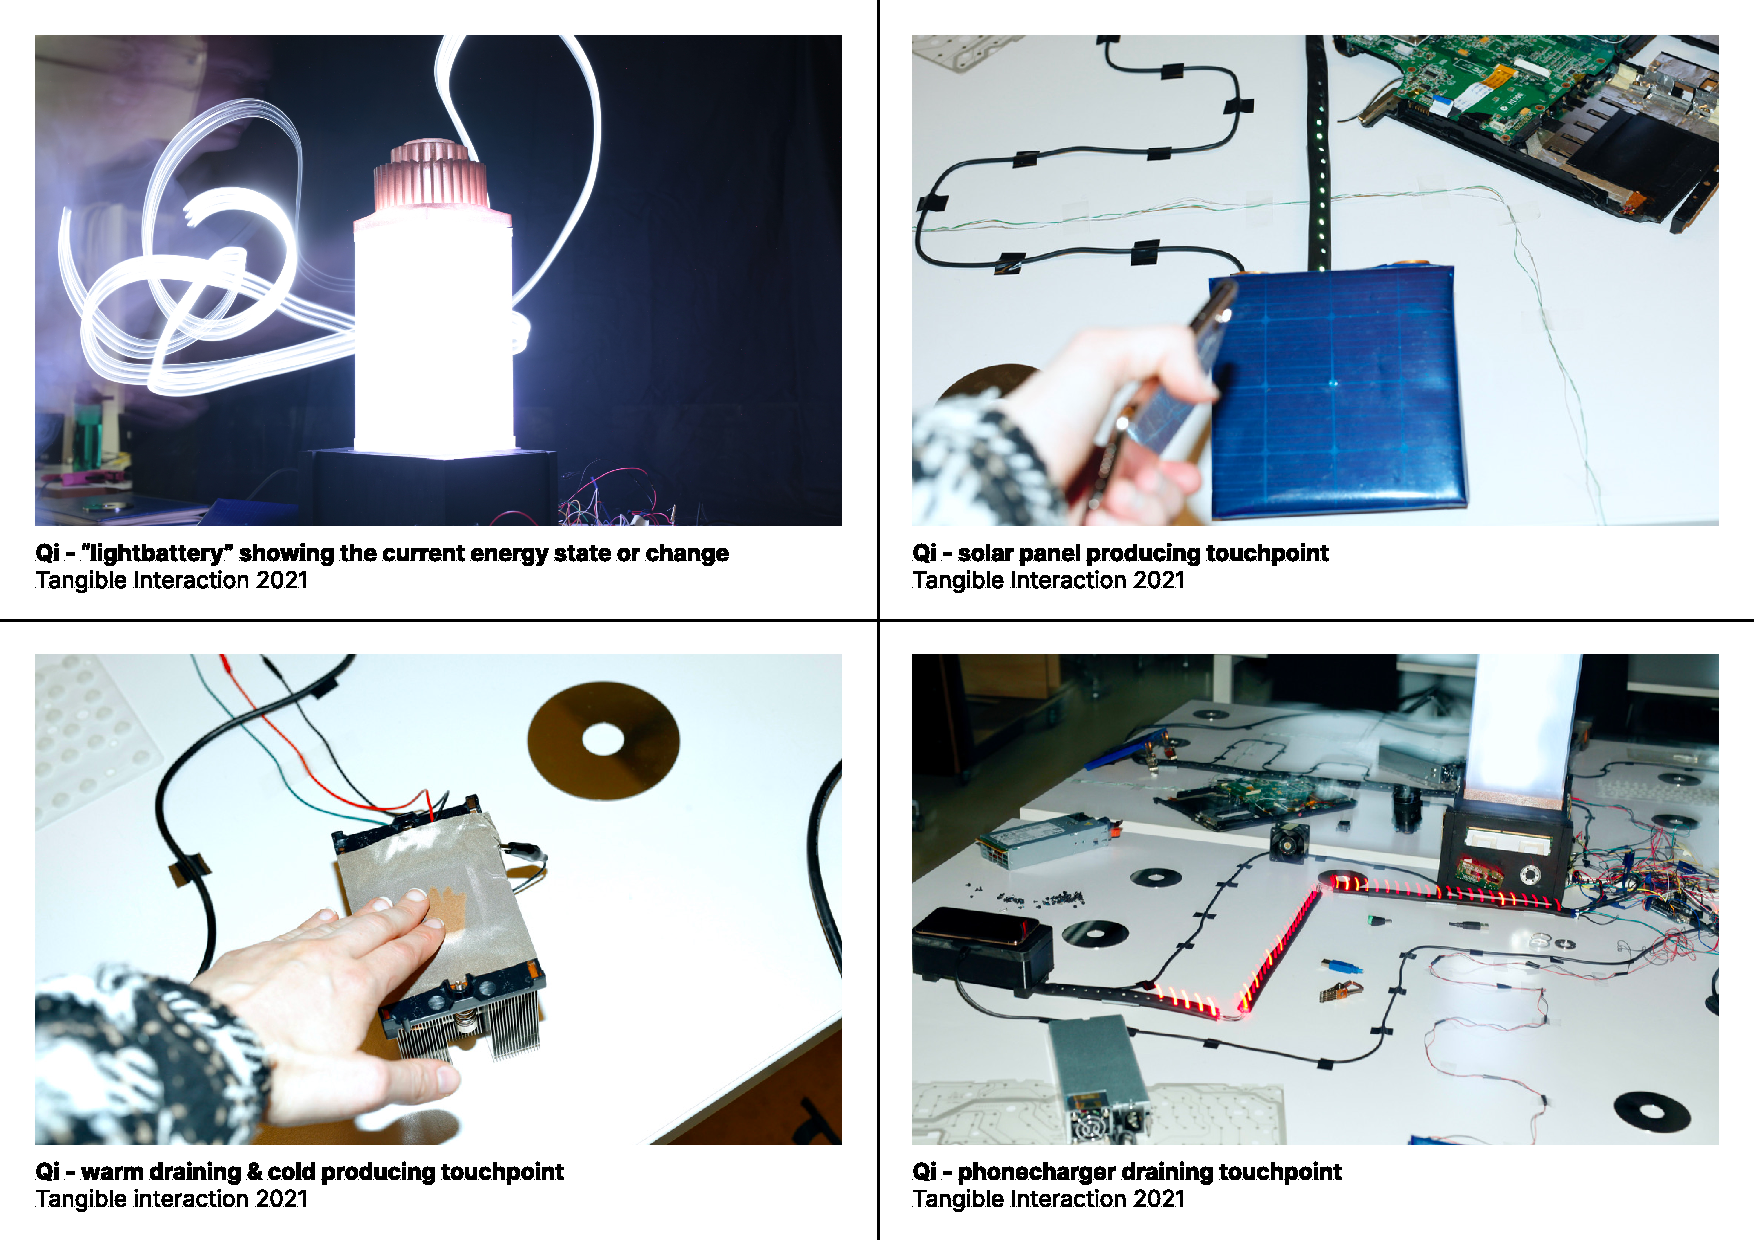
\includegraphics[width=11cm]{pictures/dataset/Qi.pdf}
\centering 
\end{figure}


\section{Observing Klimahusets narrative storytelling in-action}
\par
\emph{Observation and interview 16.02.2022}
\par

After my readings on the museum and its expository agency, I wonder what Klimahuset’s stakeholders thoughts are on their agency? And their position toward whether or not they have a subjective or objective expository agency? What are the cultural attitudes, decisions, views and stances the agents involved in designing the climate exhibition in Klimahuset, took before they decided to do the act of exposing? What cultural function does the objects on display in Klimahuset pose? 

Some of these questions can already kind of be elaborated for, from initial reading on internal documents that I have gotten access through collaborating partners in Klimahuset, as well as from conversations with stakeholders from Klimahuset last semester through the workshop, mail correspondence and mini-exhibition. As accounted for in Klimahusets founding documents, their vision/ purpose of the museum is as follows:
To give the visitors an understanding of the most important climate processes that affect the living conditions on Earth so that they are able to develop their own views on climate change, take part in climate discussions or act in other ways in relation to the topic.
Visitors must gain an understanding that natural conditions also affect social structures and culture.
	
Building on Mieke Bal’s narrative analysis on cultural imperialism in museums, say we look at Klimahuset as an ethnographic museum with the expository agency to display installations, objects and data related to the climate crisis. And with a distinct and clear target group being children aged 10-14. Is Klimahusets agency and vision an attempt to display the climate crisis as a current/ ongoing discourse with the function to educate and stimulate critical reflections on current societal norms and ways of living, or is the agency to define and lay up cultural change, to a more sustainable way of living? Maybe both? If so, then comes the question if the museums cultural stakeholders, with this expository agency, are they cultural moralists? Especially because their whole museum exhibition are designed to engage children aged 10-14, though welcoming all age groups, raises the question if the museum and exhibition design in itself potentially have any moral imperialistic function as well, as to who the discourse (the climate crisis) is relevant for. 
Asked the klimaverter about  this, need to do some structural analysis of some sort….

\begin{figure}[H]
\includegraphics[width=13cm]{pictures/elever_i_klimahuset.png}
\centering 
\end{figure}

Med en klimavert til stede får man bedre hjelp og en form for retning til å “lese” installasjonene, som støtter deg når du senere går gjennom avdeling for avdeling. 
Man blir stilt spørsmål som er knyttet til faktiske ting, som for eksempel i video-atriet sier klimavert; jeg er 160cm høy, hvor høy tror dere denne veggen er?
Etter litt håndsopprekning får vi vite at dersom Grønlandsisen smelter vil havet stige like høyt som det den veggen er. Det er tankevekkende og setter inntrykk!

Her blir man også litt senere spurt: ser dere vær eller klima? et åpent spørsmål som setter i gang en god diskusjon på forskjellen mellom vær og klima, med fokus på hvordan vær påvirker klima. Dette blir forklart at mange blander og tenker at vær og klima er det samme, og at klimaforandringer og værforandringer ikke er det samme. Her får noen elever aha-øyeblikk.


Et annet eksempel er isbiten inne i “den naturlige avdelingen”.  Først får elevene i oppgave å finne noe i området som påvirker klimaet naturlig. Senere når det blir tatt en liten runde spør verten; har alle tatt på isbiten? For så å gå videre til å forklare hvordan menneskelig påvirkning påvirker klimaet. “For eksempel har deres varme hender bidratt til å smelte litt av isbiten her i Klimahuset”. Dette er også tankevekkende og setter inntrykk!


Ice Cube: a good example of a meaningful exp. !!!


\section{Interview with a concept developer from Munch}
\par
\emph{date date date}
\par




\part{Review/ Evaluation }
\chapter{Analysis}

\section{Narrative workshop dataset}



\section{Museum visit dataset}

Over the course of this thesis, my research buddies and I have visited in total 10 exhibitions from 7 different museums in Oslo. From these museum visits, we have documented 22 interactive installations that forms the dataset used for analysis and similar investigations in our respective thesis's. 

\begin{figure}[H]
\includegraphics[width=12cm]{pictures/dataset/datasett_oversikt.jpeg}
\centering 
\end{figure}

I think this is basic qualitative analysis?

Måten jeg har gått frem på ved bruk av dette datasettet, sett opp mot mine utvalgte teorier, har vært en form for deduktiv systematisk prosess. Det vil si at jeg til å begynne med har systematisert og kategorisert installasjonene opp mot hver teori; feks som jeg har gjort her fra en av de interaktive installasjonene på klimahuset haar jeg

\subsection{"data laundering"}
Write out:
\begin{itemize}
    \item explain why munch shadows is analysed as one. and only weighted as one. and how that affects the dataset.
    \item discuss how the amount of tangible installations affect the dataset
    \item discuss the analog-tangible vs interactive-tangible installations (ice cube, munch peepholes and discovery table)
\end{itemize}

\begin{figure}[H]
\includegraphics[width=11cm]{pictures/dataset/heatmap.jpg}
\centering 
\end{figure}


\section{First iteration: seeing the bigger picture}

I started the first analytical iteration by sorting the dataset into the three theories I base my understanding of meaningfulness on; \emph{Hybrid place, place as a dialogue} and \emph{Sense-making strategies}. I made one table for each theory, where the frameworks's principles/ and dimensions formed the columns and the 22 different installations the rows. I then went through each installation and plotted in whether or not the installation fulfilled the principle/ dimension. Categorising it this way opened up for looking at the dataset in correlation with each theory separately, making it possible to see overall trends in the dataset according to the theories. Another


respective theory from a birds-eye, holistic, perspective, but it will also work as a quick-reference guide for the second analysis iteration when I'm trying to merge the three theories and/ or finding new relationships between the data across the theories.

The categorisation of the data is highly subjective, but theoretically grounded, based on my personal experience with- and interpretation of the installations and knowledge of the museum institution the installation was part of. I have also chosen to merge all the Munch - \emph{Shadows} installations as one, because they are a part of the same exhibition and do not differ in their interactive qualities. Because of this, the dataset used for this analysis shrinked from 22 to 16. This choice of merging the \emph{Shadows} installations was made in the process of fitting the installations into the theory's principles/ dimensions, when I saw that they all checked the same boxes. 


\begin{figure}[H]
\includegraphics[width=13cm]{pictures/dataset/analysis_tables.png}
\centering 
\end{figure}

After mapping the installations in the tables, it opened up for crunching the first numbers. In this iteration I want to see the dataset from a holistic view. Abstracting from the details and seeing how the installations map up in the bigger picture. To do this I needed a diagram that could compare the different principles up against eachother. I chose to create radar charts to do this, and made a radar chart for each theory. 

\begin{figure}[H]
\includegraphics[width=13cm]{pictures/dataset/analysis_radars.png}
\centering 
\end{figure}

\emph{"Findings"}
\par

What I have learned by looking at the radar charts so far is how the different theories fulfill, or complement eachother. The way I have gone forward in looking at the radar charts is as following:
\par I'll start by looking at the hybrid place radar chart, noticing how the personal and physical dimension is fulfilled, while the social and cultural dimension is very little fulfilled. What does this mean? According to the Norwegian museum policy strategic thinking, it is wanted that museums transition from the personal dimension to the more social and cultural dimension. The fact that installations in my analysis shows presence in the physical dimension is positive, in terms of enabling the personal dimension, experience-wise, to involve more tangible or at least dynamic experiences in the museum space.
\par Then, if we shift focus for a second to look into the sense-making radar chart, we see that one of the corners that is fulfilled by almost all installations in this analysis - support for sharing is fulfilled. How come, that even though the social dimension is not fulfilled while almost all installations, in terms of sense-making have good support for sharing? 

\par Then again, we can look at what dialogic qualities the installations turns out to have little "relationalness", which is a dialogic principle/ quality that involves the Docents in the museum for example, or relational qualitites.





\chapter{Discussion}
In this chapter we look back at the thesis project and discuss how one can design for meaningful interactive experiences in a museum space.

\section{The nature of the contributions}
This thesis has two research contributions, one theoretical and one practical:
\begin{itemize}
    \item Theoretical contribution: framework used to identify and analyse dialogic relations between visitor and interactive installations.
    \item Practical contribution to HCI/ IxD field: dialogical installation patterns that objectify meaningfulness as a quality that you can design for.
\end{itemize}


The framework: A resource for the designer to judge the degree of dialogic instalaltion design, dialogic visitor experience and museum space hybridness. Together, they synthesise an understanding of meaningfulness rooted in the museum/ exhibition artefacts supporting or extending dialogic behaviour: conversations, reflections etc, between the visitor and installation. But also from visitor-to-visitor, or groups, walking through the museum narrative. This would be a good fit for museum disseminating discourses that demand/ wish to stimulate dialogue as one of the main "things" the visitor should "sitte igjen med" after the museum visit. I would argue this is relevant for museums disseminating contemporary discourses, like the climate crisis, to ensure partaking in the public debate. And help manifest the museum space as a modern place being able to "følge med i tiden".. 

We have shown how the framework can be applied to analyse a specific exhibition addressing one discourse. But also seen how the framework work across different installations and exhibitions addressing different discourses. Doing an analysis as such could prove useful for a city planning a new museum, seeing how the museums differ in terms of meaningfulness and stimulating dialogic behaviour. Perhaps new museums can fill, or complement, a gap that the existing museums does not. 

What is nice with the framework is that it is designed for interactive installations- and artefacts, but it allows for "analogue" artworks or artefacts parts of the exhibition to take part in the analysis as well. If the curator is looking at the exhibition as a whole, it would make sense to involve all parts of the journey. E.g., Klimahuset and ice cube. 

\section{Contributions to the field}

This thesis contribution is valuable for the broader HCI community interested in designing or analysing public installations in museums. By presenting a theoretical framework used to both identify and analyse dialogic relations between visitor and interactive installations. 

HCI is increasingly interested in considering how technology-use impacts the human experience of meaning \autocite{kaptelinin_technology_2018}, \autocite{light_design_2017}, as well as how to design for and foster meaningful user experiences \autocite{grosse-hering_slow_2013}, \autocite{Hassenzahl_Moments_2013}.


Literature concerned with interactivity and meaningful engagement with visitors [ \autocite{mccarthy_place}, \autocite{ciolfi_designing_2012}], are often written in the context of heritage museums. While this thesis contribution is derived in the context of different museum fictions; art (MUNCH), science (Teknisk Museum), and natural history (Klimahuset). 


Literature agrees on museums having become a place for education and learning, dialogue and debate \autocite{narrative_sitzia}, \autocite{hein_1998}, \autocite{hooper_1994}, \autocite{Roberts_1997}. An interest that is also shared politically, as evident in \autocite{melding23}. 

Surveys from, for example, the USA show that museums score higher on trust than other institutions, such as media and government agencies, and that credibility of museums continues to increase during the pandemic \autocite{impact_2020}. As important actors in the public discourse, it is crucial for museums in the future that they defend this position and further develop it. It is essential to secure a position where a room is created for different opinions to meet and break and counter the emergence of echo chambers, conspiracy theories, and false news \autocite[p. 41]{melding23}.


Then comes the question, what does the interactive artefact or installation represent? As far as my literature search goes, there is not so much attention given to the role of the interactive artefact or installation in the HCI community. The community seem to be more interested on what makes the installation engaging, and how it can provide an engaging experience for the visitor and groups as evident in the works of \autocite{hornecker_learning_2006}, and \autocite{ciolfi_designing_2012}.

"For the last several years the HCI community has been undergoing a broadening of scope from usability to user experience; making things that improve the quality of people’s lives across a range of contexts. Our community has recognized that in addition to making products that make people more efficient and effective, we need to learn to make things that affect people in a variety of ways." \autocite[p. 395]{zimmerman_designing_2009}. 

There has been increased interest in the field of visitor studies and museum research in the details of visitor behaviour in museums, which is what the research done on indexing contributes to \autocite[p. 41]{hornecker_to-and-fro_2016}


"Thanks to the development of ubiquitous and pervasive technologies, research focusing on the design of novel interactive artefacts has recently become more concerned with studying and understanding the spatial properties of the world" \autocite[p. 159]{hybridplace_ciolfi}

In Ciolfi and McCarthy’s opinion, frameworks that have been made to guide the design of interactive museum exhibitions developed in the field of museums studies, underplay aspects of visitor’s active sense making and interpretation. They argue that most practical and conceptual contributions from both museum studies and interaction design have fallen short of their potential to reflect on and design technologically mediated museum experiences partly because of the underdeveloped or under-articulated conceptualisations of visitor experience with which they work \autocite[p. 248]{mccarthy_place}


\textbf{USE OF PATTERNS:} "My use of design patterns deviates fairly widely from their intended purpose of documenting and making explicit design conventions. The design patterns from the individual products are not particularly valuable to other designers, because they do not document a general solution. However, they worked very well to illuminate the link between design intention (application of product design theory) and the designed artifact, allowing the similarities in the application of theory across the very different design projects to be seen." \autocite[p. 402]{zimmerman_designing_2009}.


\subsection{Generating knowledge through analysis of design}
As a field, HCI must answer what sorts of knowledge outcomes can come from objects in (art and) design projects; if we cant, we cannot legitimize RtD as a way of doing HCI research. Bardzell offer theoretical support for RtD by arguing that to legitimise and make use of research through design as \emph{research}, HCI researchers need to explore and clarify how RtD objects contribute to knowledge \autocite[p.2093]{bardzell_immodest_2015}. Along these lines, Bardzell et.al argue that while the \emph{intentions} of the object's designer are important and annotations are a good mechanism to articulate them, the critical reception of objects can be equally generative of RtD's knowledge impacts \autocite[p. 2093]{bardzell_immodest_2015}. Bardzell et.al. investigate RtD in its relation to the production of knowledge; specifically, \emph{how design objects are knowledge producers both for those that encounter them and those that design them} \autocite[p. 2093]{bardzell_immodest_2015}. To explore how a detailed critique might work when we understand objects as knowledge producers offering to the viewer the possibility to engage in meaning-making practises unfolding a range of complex and multi-faceted views, Bardzell et. al offer a multilevel analysis of a critical design fiction. \autocite[p. 2094]{bardzell_immodest_2015}.

The primary purpose of this thesis has been to contribute with knowledge that makes visible dialogic relations between interactive installations and visitor-experience in the museum space, to attempt to answer how one can design meaningful interactive experiences in a museum space. "By making different things intended to address the same problematic situation, RtD can reveal design patterns \autocite{Alexander_book} around problem framings, around specific interactions, and around how theory can be operationalized" \autocite[p. 178]{zimmerman_research_2014}.


\section{Disposition}

"Overall this paper contributes to HCI research on the technological augmentation of heritage sites both by addressing a seldom-studied domain, (...) This contribution is also of value for the broader HCI community interested in public installations, by showing how a thoughtful assembly of different interactional elements (from mobile applications, to standalone pieces and low-tech tangible components) can engage visitors and engender the establishment of personal connections." \autocite{ciolfi_designing_2012}


\begin{itemize}
    \item Contribution 1: by putting three theoretical approaches together we have made a framework (chapter 6) that proposes a new way of designing for meaningfulness. The new framework have been used to guide datagathering (chapter 8), and through analysis we have proven how we can derive a list of patterns. The framework have therefore proved useful as a tool for designers following a whole iteration in a design process.
    
    
    \item Contribution 2: the list of patterns. They can be used (by designers) in early conceptual stages as inspiration or starting points for dialogic installation designs. 
    \item These contributions is the answer to; \emph{How one can design for meaningful interactive experiences in a museum space.}
    \item
    
     \item These contributions + literature review (chapter 2), is the answer to; \emph{How can one (...) in a museum space that addresses \textbf{sustainability}}. Sustainability represents a contemporary discourse that demand active discussion and engagement. Dialogic installations are my proposal of a way that museums can address contemporary issues without being cultural moralists, simply facilitating for reflection, and dialogue in the museum, as the  in the time after the visit. 
    \item Discuss dialogic installation design up against the field's current "state" or contributions of something like that.

\end{itemize}


\section{Research as a creative, generative process (or something like this?)}
This study reflects the challenging "climate" where design research meet installation design, museums facilitating attitude change and sustainability as a contemporary, and complex (!), discourse.

At the time, I was unaware of the methodological and practical consequences of structuring my understanding through three different theories, while doing research through design. It has been a time-consuming effort to support this methodological choice and find support in the literature as to how this way of doing RtD has generated knowledge. 





\begin{itemize}
    \item Contributions to the field (HCI, interaction design, museum studies). HCI/ I.D. --> RtD as a generative and creative process. Museum studies: an attempt to objectify interactive meaningful qualities in museum spaces
    \item Discuss my term "meaningfulness" up against the field's definition of meaningfulness. 
    
    \item Documentation --> the researchers basis for contributions (\emph{the research}). In this study, the documentation have played a creative and generative role - just as much as being sound (valid) for scientific purposes like analysis. 
    \item RQ ---> in this study used as a "creative driver" for the design process. Seen as something "alive", fluid, that drives conceptual exploration just as much as the scientific exploration/ inquiry.
    \item Science is a generative and creative process. This study aim to strengthen the notion that design has a place in research, agreeing with Frayling and RtD literature saying that science + design = true. 

\end{itemize}




\chapter{Conclusion}

This thesis has discussed how one can design meaningful interactive experiences in a museum space that addresses sustainability by analyzing a selection of interactive installations and exhibition spaces in local museums. In addition, the thesis has considered the development and shift in museology practice against ubiquitous computing and design as meaning-making in museums, aimed to forge a stronger connection between the HCI/ IxD field and museum studies. This has been conceptually explored by using sustainability and the Anthropocene as a discourse representative of a contemporary ongoing public debate or topic that museums being institutions of knowledge, have incentive and means to engage in by communicating the science of climate change. 

The first contribution is a framework that can be used to identify and analyse dialogic relations between visitor and interactive installations. The second contribution is a list of 21 dialogical installation patterns that function to objectify meaningfulness as a quality that you can design for.



\backmatter{}
\printbibliography[nottype=online]

% https://no.overleaf.com/learn/latex/Bibliography_management_in_LaTeX

% \printbibliography[type=article,title={Articles only}]
 \printbibliography[type=online,title={Web only}]


% \appendix
% \chapter{Appendix}
% \section{Three approaches to place-centred design}

% Hybrid place dimensions reference
% Place as dialogue reference

\section{Methodology & Process}
% zimmerman and Forlizzi (2004), knowledge opportunity map in the design process

\subsection{Klimahuset stories workshop dataset}



\subsubsection{Results from the Narrative Workshop}
\begin{figure}[H]
\includegraphics[width=12.5cm]{pictures/process/workshop_results.png}
\caption{Results from the Narrative Workshop described in section 8.2: Investigating narratives and storytelling with Klimahuset.}
\centering 
\end{figure}

\subsubsection{Concept pitches that were not realized}

\begin{figure}[H]
\includegraphics[width=12.5cm]{pictures/appendix/oldphone_pitch.png}
\caption{}
\end{figure}

\begin{figure}[H]
\includegraphics[width=12.5cm]{pictures/appendix/keypad_pitch.png}
\caption{}
\end{figure}



\section{Analysis}
This section contains 

\begin{figure}[H]
\includegraphics[width=12.5cm]{pictures/dataset/heatmap.jpg}
\caption{Heatmap version 1, Munch shadows is weighted as one}
\end{figure}

\section{Datagathering: observation guide}
\begin{figure}[H]
\includegraphics[width=13cm]{pictures/appendix/datagathering.png}
\centering 
\end{figure}

\section{Datagathering: interview guide}
\section{Dataset: Interactive Installations}

\begin{figure}[H]
\includegraphics[width=13cm]{pictures/dataset/munch_1.png}
\centering 
\end{figure}

\begin{figure}[H]
\includegraphics[width=13cm]{pictures/dataset/munch_2.png}
\centering 
\end{figure}

\begin{figure}[H]
\includegraphics[width=13cm]{pictures/dataset/munch_3.png}
\centering 
\end{figure}

\begin{figure}[H]
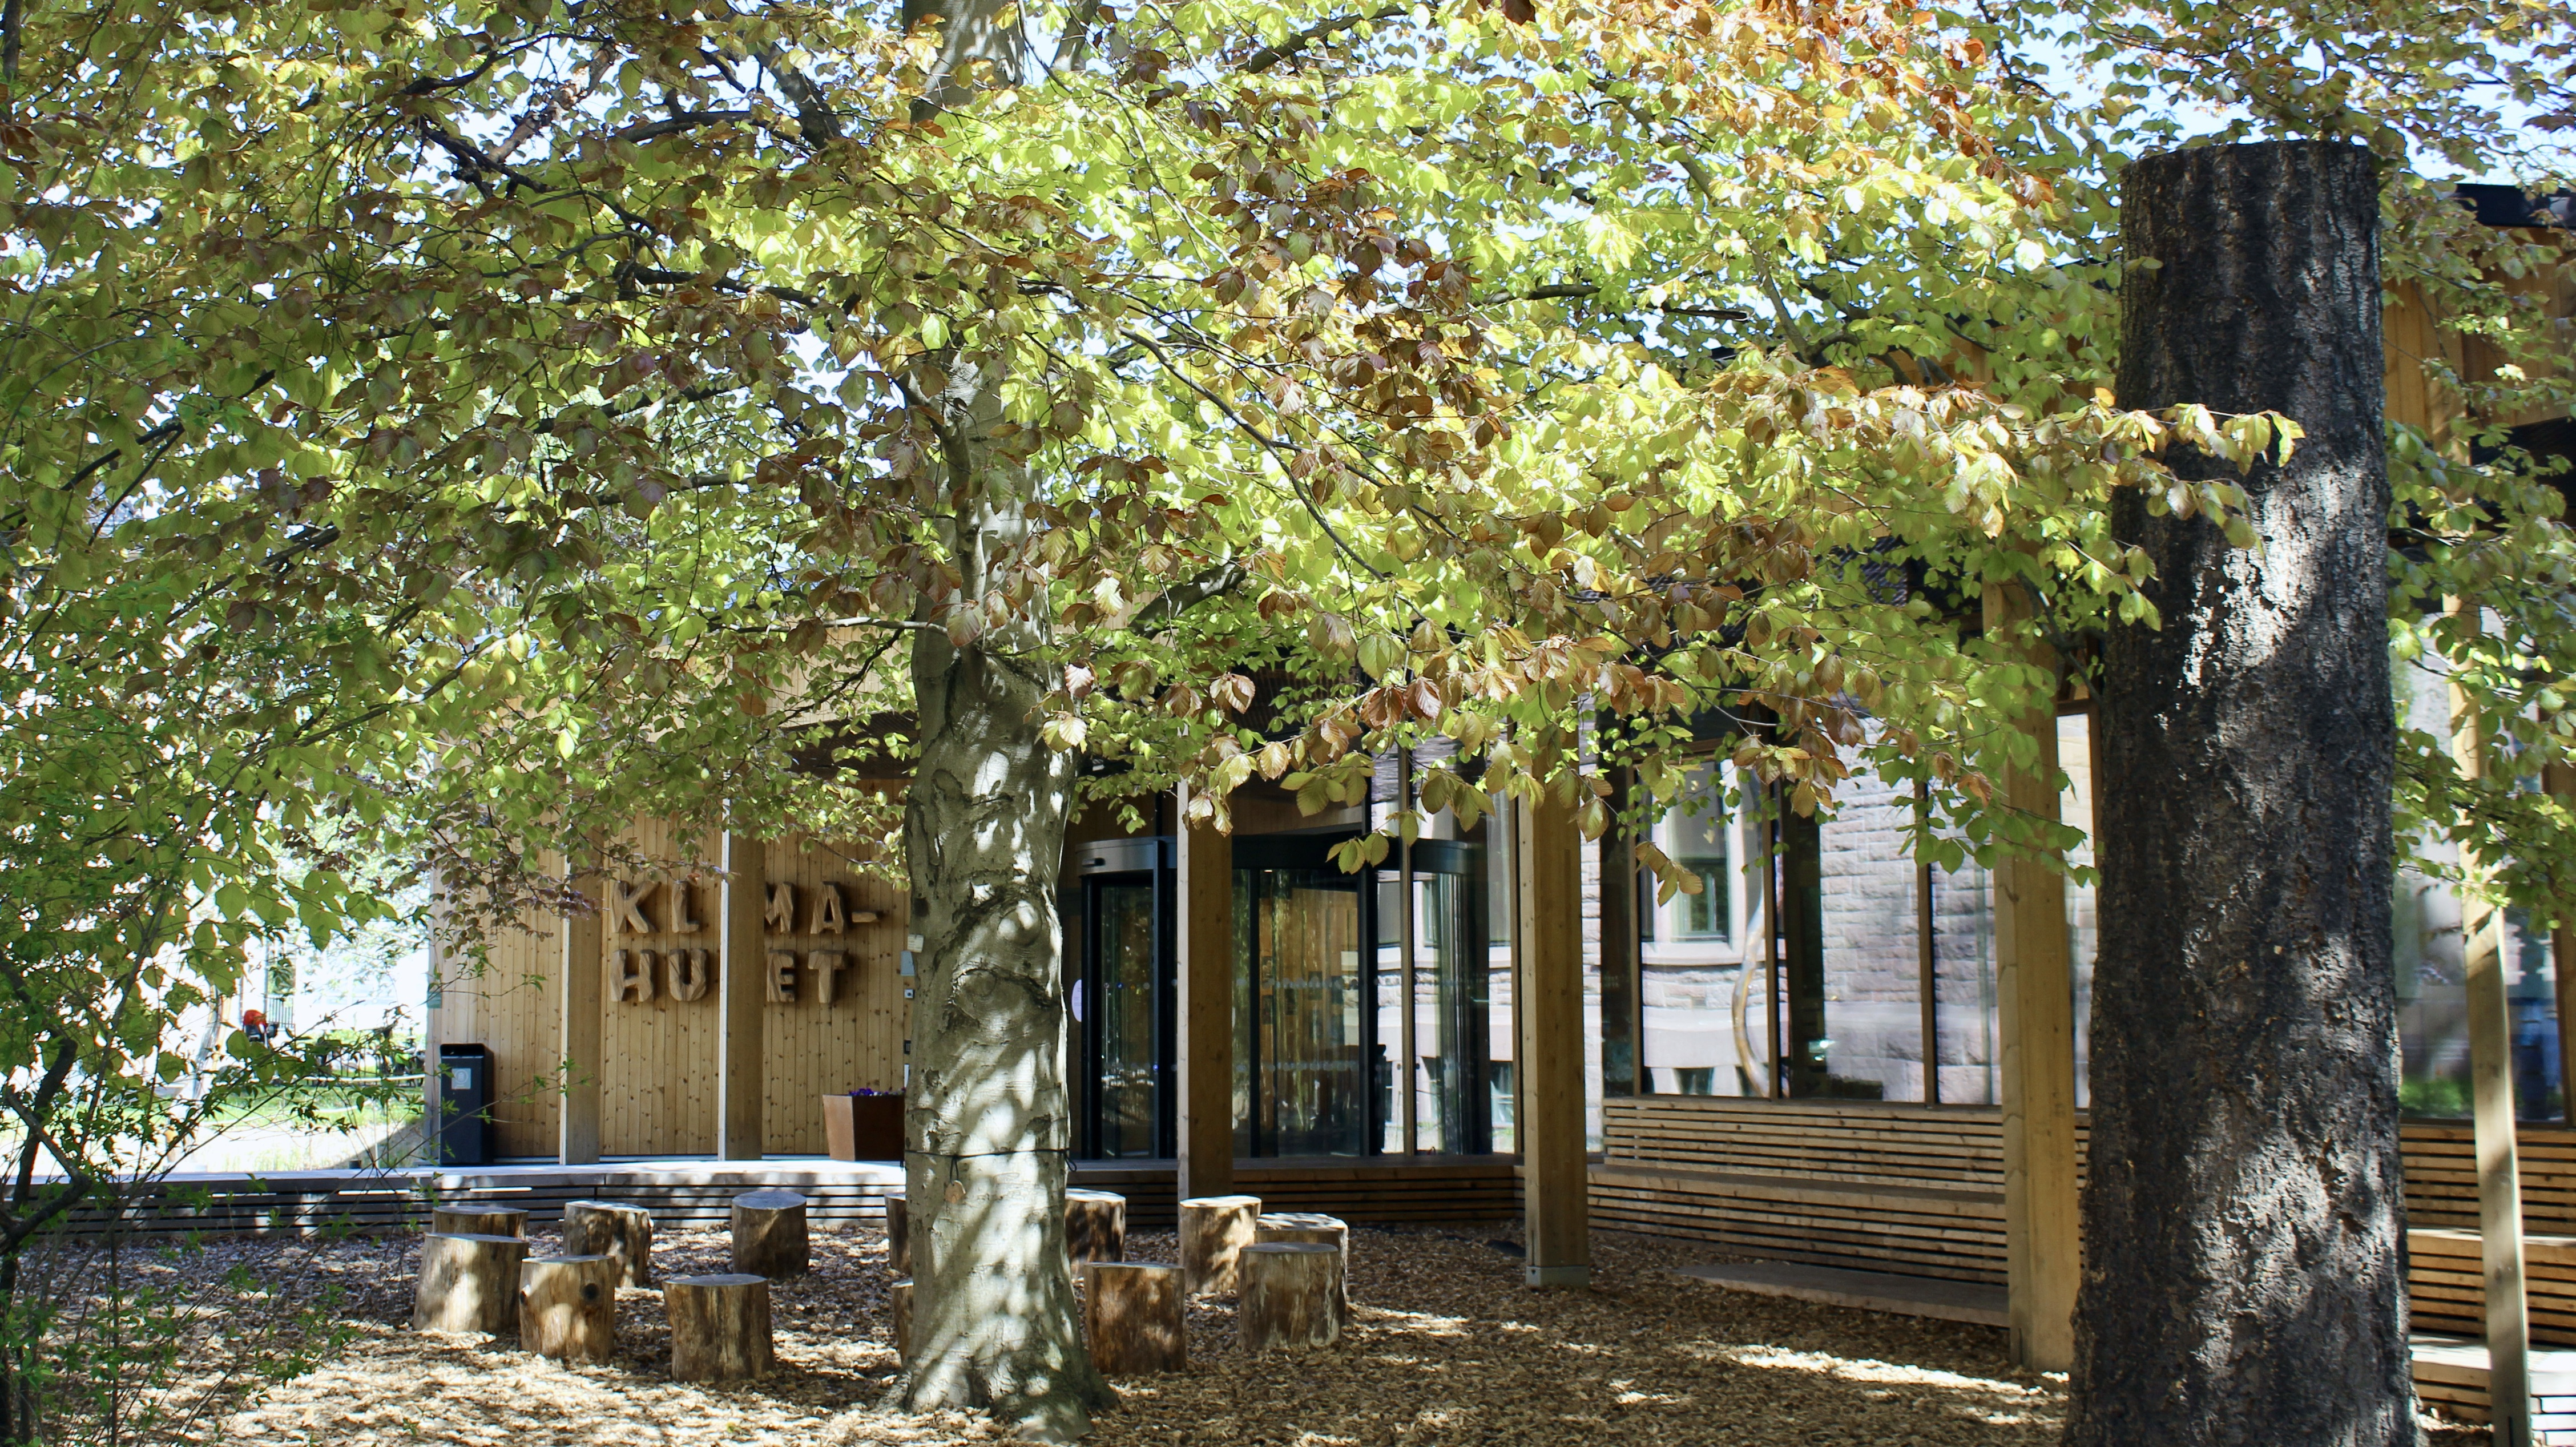
\includegraphics[width=13cm]{pictures/dataset/klimahuset.png}
\centering 
\end{figure}

\begin{figure}[H]
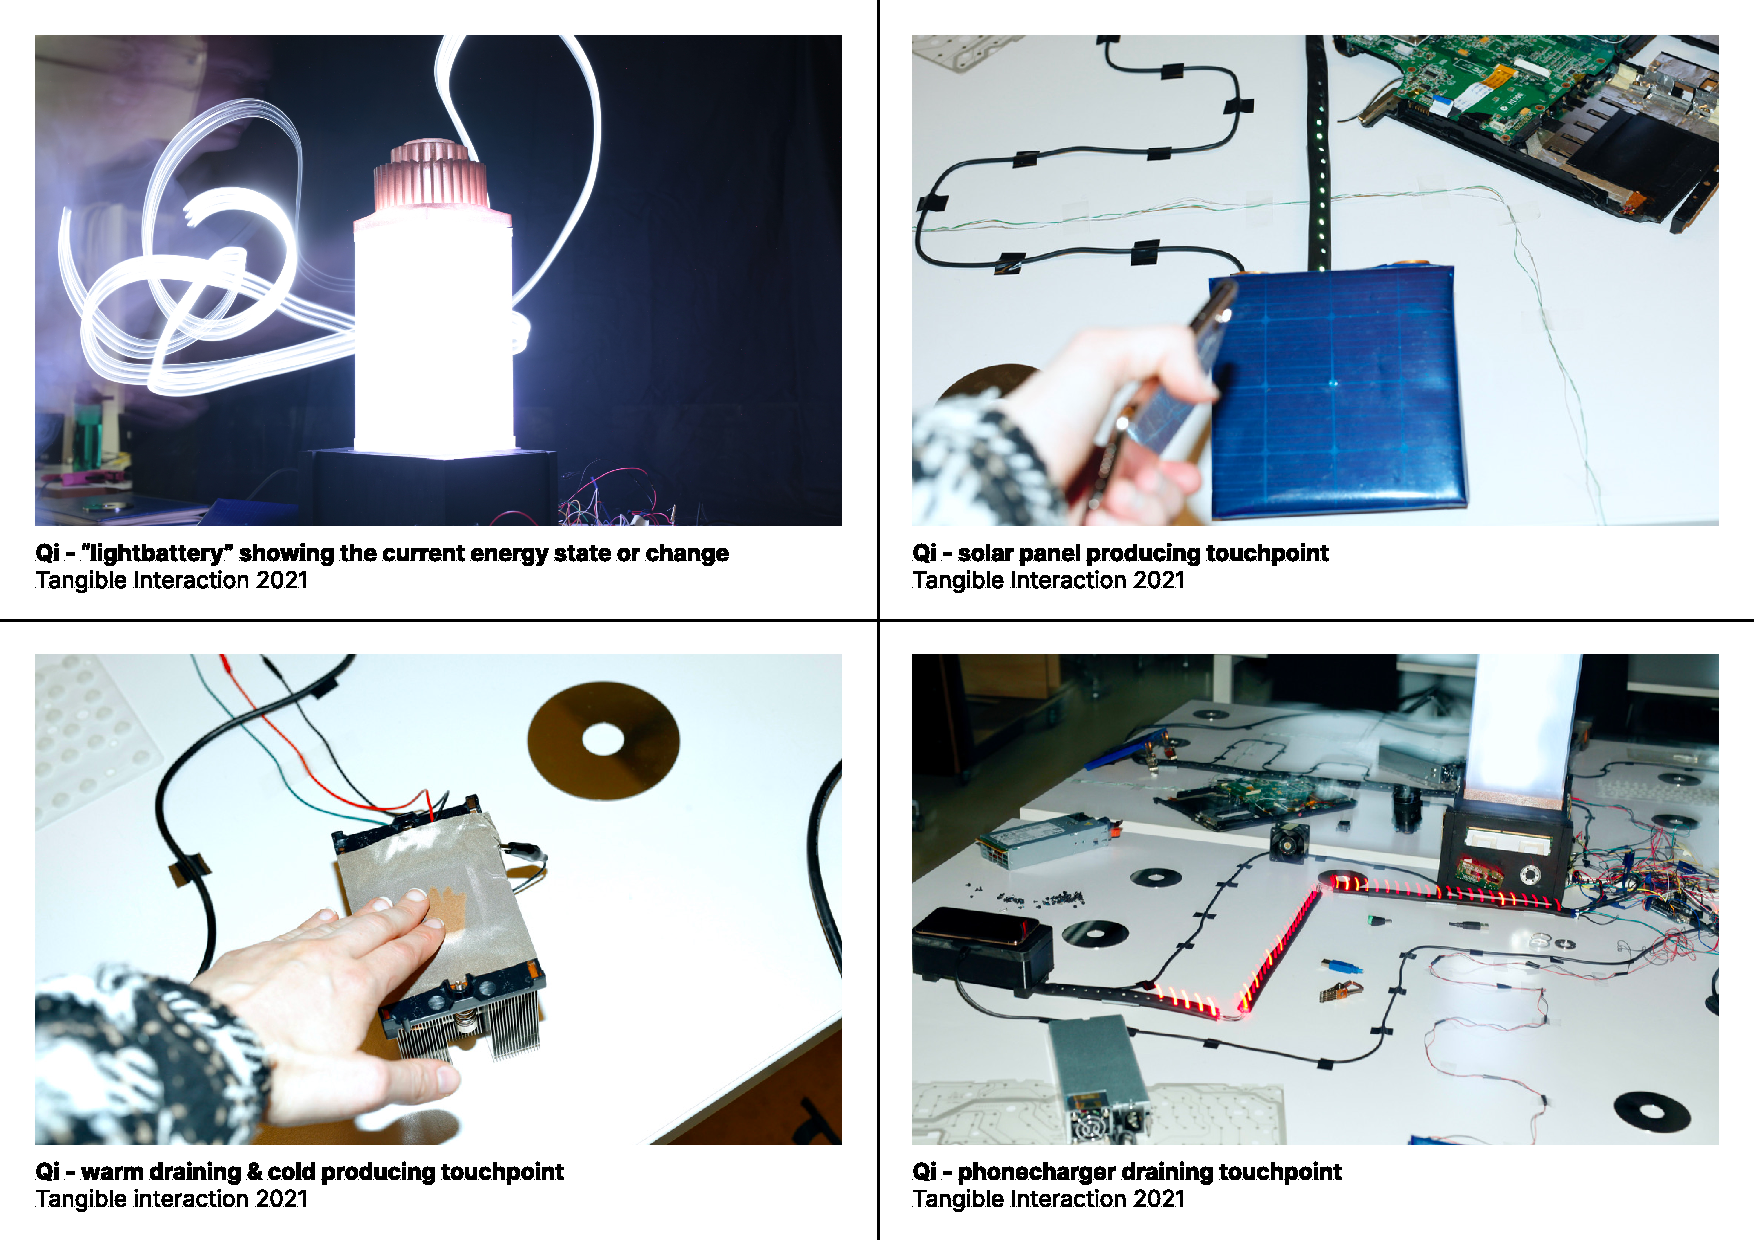
\includegraphics[width=13cm]{pictures/dataset/Qi.pdf}
\centering 
\end{figure}

\begin{figure}[H]
\includegraphics[width=13cm]{pictures/dataset/tangible.png}
\centering 
\end{figure}

\begin{figure}[H]
\includegraphics[width=13cm]{pictures/dataset/yuko_mohri.png}
\centering 
\end{figure}

\section{Consent forms}

\begin{figure}[H]
\includegraphics[width=12.5cm]{pictures/appendix/Samtykkeskjema_klimahuset.pdf}
\caption{Consent form for employees at Klimahuset}
\end{figure}

\begin{figure}[H]
\includegraphics[width=12.5cm]{pictures/appendix/Samtykkeskjema Munch.docx.pdf}
\caption{Consent form for employees at Klimahuset}
\end{figure}



\end{document}